% ============================================================
%  PREAMBLE — compile with pdfLaTeX + biber
% ============================================================
\documentclass[12pt,a4paper]{report}

% ── Encoding & Language ──────────────────────────────────────
\usepackage[utf8]{inputenc}
\usepackage[T1]{fontenc}
\usepackage[english]{babel}

% ── Page Layout ──────────────────────────────────────────────
\usepackage{geometry}
\geometry{
  a4paper,
  top=2.5cm,
  bottom=2.5cm,
  left=3cm,
  right=2.5cm
}

% ── Typography & Spacing ─────────────────────────────────────
\usepackage{setspace}
\onehalfspacing
\usepackage{parskip}
\usepackage{ragged2e}

% ── Mathematics ──────────────────────────────────────────────
\usepackage{amsmath}
\usepackage{amssymb}

% ── Graphics & Colors ────────────────────────────────────────
\usepackage{graphicx}
\usepackage{xcolor}
\usepackage{tikz}

% ── Tables ───────────────────────────────────────────────────
\usepackage{array}
\usepackage{booktabs}
\usepackage{tabularx}
\usepackage{adjustbox}
\usepackage{float}

% ── Boxes & Frames ───────────────────────────────────────────
\usepackage{mdframed}

% ── Headers & Footers ────────────────────────────────────────
\usepackage{fancyhdr}

% ── Section & Chapter Formatting ─────────────────────────────
\usepackage{titlesec}
\titleformat{\chapter}[block]
  {\normalfont\Large\bfseries}{}{0em}{}
\titlespacing*{\chapter}{0pt}{0pt}{20pt}

% ── Hyperlinks ───────────────────────────────────────────────
\usepackage{hyperref}
\hypersetup{
  colorlinks=true,
  linkcolor=blue,
  citecolor=blue,
  urlcolor=blue,
  pdfborder={0 0 0},
  hyperindex=true,
  pageanchor=true,
  linktoc=all
}

% ── Bibliography ─────────────────────────────────────────────
\usepackage[
  backend=biber,
  style=authoryear,
  natbib=true,
  maxcitenames=2,
  uniquelist=false,
  hyperref=true,
  backref=true
]{biblatex}
\addbibresource{references.bib}

% ── Make the ENTIRE citation (author + year) clickable ───────
\DeclareCiteCommand{\cite}
  {\usebibmacro{prenote}}
  {\usebibmacro{citeindex}%
   \printtext[bibhyperref]{\usebibmacro{cite}}}
  {\multicitedelim}
  {\usebibmacro{postnote}}

\DeclareCiteCommand{\parencite}[\mkbibparens]
  {\usebibmacro{prenote}}
  {\usebibmacro{citeindex}%
   \printtext[bibhyperref]{\usebibmacro{cite}}}
  {\multicitedelim}
  {\usebibmacro{postnote}}

\DeclareCiteCommand{\textcite}
  {\boolfalse{cbx:parens}}
  {\usebibmacro{citeindex}%
   \printtext[bibhyperref]{\usebibmacro{textcite}}}
  {\ifbool{cbx:parens}
     {\bibcloseparen\global\boolfalse{cbx:parens}}
     {}%
   \multicitedelim}
  {\usebibmacro{textcite:postnote}}

\DeclareCiteCommand{\citet}
  {\boolfalse{cbx:parens}}
  {\usebibmacro{citeindex}%
   \printtext[bibhyperref]{\usebibmacro{textcite}}}
  {\ifbool{cbx:parens}
     {\bibcloseparen\global\boolfalse{cbx:parens}}
     {}%
   \multicitedelim}
  {\usebibmacro{textcite:postnote}}

\DeclareCiteCommand{\citep}[\mkbibparens]
  {\usebibmacro{prenote}}
  {\usebibmacro{citeindex}%
   \printtext[bibhyperref]{\usebibmacro{cite}}}
  {\multicitedelim}
  {\usebibmacro{postnote}}

% ============================================================
\begin{document}

% ── FRONT MATTER (roman page numbers) ───────────────────────
\pagestyle{empty}
\pagenumbering{roman}


% ============================================================
%  PAGE 1 — COVER PAGE
% ============================================================
\begin{titlepage}

% Page double border
\begin{tikzpicture}[remember picture, overlay]
  \draw[line width=2pt]
    ([shift={(0.55cm,0.55cm)}]current page.south west)
    rectangle
    ([shift={(-0.55cm,-0.55cm)}]current page.north east);
  \draw[line width=0.5pt]
    ([shift={(0.7cm,0.7cm)}]current page.south west)
    rectangle
    ([shift={(-0.7cm,-0.7cm)}]current page.north east);
\end{tikzpicture}

% Watermark
\begin{tikzpicture}[remember picture, overlay]
  \node[opacity=0.07] at (current page.center)
    {
\includegraphics[width=0.68\paperwidth]{picture/logo/logo.png}};
\end{tikzpicture}

  % ── Arabic header ───────────────────────────────────────
  \begin{center}
    {\small\bfseries People's Democratic Republic of Algeria}\\[1pt]
    {\small\bfseries Ministry of Higher Education and Scientific Research}
  \end{center}

  \vspace{3pt}
  \noindent\rule{\linewidth}{0.5pt}
  \vspace{4pt}

  % ── University row ──────────────────────────────────────
  \begin{center}
  \begin{tabular}{p{0.34\linewidth} c p{0.34\linewidth}}
    \raggedright
    {\small Universit\'e Badji Mokhtar -- Annaba\\
             Badji Mokhtar -- Annaba University} &
    \raisebox{-0.45cm}{%
      
\includegraphics[height=1.7cm]{picture/logo/logo.png}} &
    \raggedleft
    {\small\bfseries Universit\'e Badji Mokhtar\\
                     -- Annaba --}
  \end{tabular}
  \end{center}

  \vspace{4pt}
  \noindent\rule{\linewidth}{0.5pt}
  \vspace{6pt}

  % ── Faculty block ───────────────────────────────────────
  \begin{flushleft}
    {\small \textbf{Faculty:} Technology}\\[2pt]
    {\small \textbf{Department:} Computer Science}\\[2pt]
    {\small \textbf{Domain:} Mathematics -- Computer Science}\\[2pt]
    {\small \textbf{Field:} Computer Science}\\[2pt]
    {\small \textbf{Speciality:} Machine Learning \& Intelligent Systems}
  \end{flushleft}

  \vspace{0.5cm}

  % ── Memoir label ────────────────────────────────────────
  \begin{center}
    {\large\bfseries Memoir}\\[4pt]
    {\normalsize Presented for the award of the \textbf{Master's Degree}}
  \end{center}

  \vspace{0.25cm}
  \begin{center}{\large\bfseries Theme}\end{center}
  \vspace{0.25cm}

  % ── Title box ───────────────────────────────────────────
  \begin{mdframed}[
    linecolor=black, linewidth=1pt,
    innertopmargin=14pt, innerbottommargin=14pt,
    innerleftmargin=18pt, innerrightmargin=18pt,
    roundcorner=4pt
  ]
    \begin{center}
      {\large\bfseries
        Leveraging Deep Learning Techniques for Advanced\\[5pt]
        Recommender Systems
      }
    \end{center}
  \end{mdframed}

  \vspace{0.55cm}

  % ── Author ──────────────────────────────────────────────
  \begin{center}
    \textbf{Presented by:} \quad Farouk Ouled Meriem
  \end{center}

  \vspace{0.35cm}

  % ── Supervisor ──────────────────────────────────────────
  \begin{center}
    \begin{tabular}{lll}
      \textbf{Supervisor:} & Samira Lagrini \quad & [Grade] \quad Badji Mokhtar -- Annaba University
    \end{tabular}
  \end{center}

  \vspace{0.45cm}

  % ── Jury ────────────────────────────────────────────────
  \begin{center}
    \textbf{Defense Jury:}\\[8pt]
    \begin{tabular}{|p{3.8cm}|p{1.5cm}|p{4.2cm}|p{2.5cm}|}
      \hline
      {[Jury Member 1]} & MCB & Badji Mokhtar -- Annaba University & President   \\ \hline
      {Samira Lagrini}  & MCA & Badji Mokhtar -- Annaba University & Supervisor  \\ \hline
      {[Jury Member 2]} & MCB & Badji Mokhtar -- Annaba University & Examiner    \\ \hline
    \end{tabular}
  \end{center}

  \vfill

  \begin{center}
    {\normalsize\bfseries University Year: 2024/2025}
  \end{center}

\end{titlepage}


% ============================================================
%  PAGE 2 — ACKNOWLEDGEMENTS
% ============================================================
\newpage
\chapter*{Acknowledgements}
\addcontentsline{toc}{chapter}{Acknowledgements}

\vspace{1cm}

First of all, I express my deepest gratitude to \textbf{Allah} for granting me
the strength and perseverance to accomplish this work.

\vspace{0.5cm}
I sincerely thank my \textbf{parents} for their unconditional love, support,
and sacrifices throughout my studies.

\vspace{0.5cm}
My heartfelt thanks go to my supervisor for their constant guidance,
availability, and valuable feedback at every stage of this work.

\vspace{0.5cm}
I also extend my appreciation to the members of the jury for their time
and careful evaluation of this memoir.

\vspace{0.5cm}
Finally, I thank all my colleagues and friends for their encouragement
and support throughout this journey.


% ============================================================
%  PAGE 3 — DEDICATIONS
% ============================================================
\newpage
\chapter*{Dedications}
\addcontentsline{toc}{chapter}{Dedications}

\vspace{2.5cm}

\begin{center}
  \itshape\large
  To my parents,\\[8pt]
  for every sacrifice they made so I could reach this day.\\[24pt]

  To my family and friends,\\[8pt]
  for their constant support and encouragement.\\[24pt]

  \upshape\normalsize\textbf{Farouk Ouled Meriem}
\end{center}


% ============================================================
%  TABLE OF CONTENTS, LIST OF FIGURES, LIST OF TABLES
% ============================================================
\newpage
\tableofcontents
\newpage
\listoffigures
\newpage
\listoftables


% ============================================================
%  GENERAL INTRODUCTION (Unnumbered Chapter)
% ============================================================
\newpage
\pagenumbering{arabic}

\chapter*{General Introduction}
\addcontentsline{toc}{chapter}{General Introduction}

% ── Context and Motivation ───────────────────────────────────
\section*{Context and Motivation}

The era of digital transformation witnesses millions of users being connected
via networks and online platforms, serving as essential components of people's
everyday lives. Various websites including E-commerce platforms have allowed
people to purchase/sell products worldwide, whereas online platforms like
Youtube facilitate instant access to numerous kinds of entertainment such as
movies, music and shows.
Because of the rapid developments that happened in the digital domain, the
amount of contents created online had a tremendously exponential growth. Such
vast amount of information available made people very difficult to make a
proper choice or obtain relevant content corresponding to user interest. Under
such overwhelming amount of choices available, user's decision making might be
impaired or confused.
The emergence of recommendation systems is to tackle with this kind of
problems. By learning the user interests and behavior, recommendation systems
can facilitate users discover desired products, services or content.
Recommendation systems contain several categories and sequential recommendation
is one of the important ones and has been considered a major research direction
in recent years. Unlike traditional collaborative filtering approaches, which
identify user interests by group similarities, sequential recommendation models
usually take advantage of user interaction history where temporal order matters,
so as to predict the next item the user will likely interact with --- such as
purchase, watch or listen to. By mining the user's past sequence of behaviors,
this kind of model has better performance in capturing dynamic user interests
and therefore better recommends relevant contents.
The booming of deep learning has been a driving force in the sequential
recommendation area in recent years. Early work based on Recurrent Neural
Networks, such as \citet{hidasi2016gru4rec}, is specifically designed for
sequences where order is important. These models capture short-term temporal
dynamics of user behavior.
Attention mechanisms and Transformer-based architectures provided a great
breakthrough. Models like SASRec \citep{kang2018sasrec} and BERT4Rec
\citep{sun2019bert4rec} capture long-range dependencies within user interaction
sequences, and both show better accuracy and scalability than previous work.
Meanwhile, Graph Neural Networks were introduced to model the global relation
of users and items over the interaction graph and to obtain rich collaborative
information that traditional sequential models could not discover.
However, these two types of methods have their respective strengths and
weaknesses. Graph Neural Networks excel in capturing the global co-occurrence
relations in the interaction graph but are weaker in modelling the local
sequential context of users. Sequence-based Transformer models are strong in
modelling a user's recent context information and preferences, but fail to
capture global information.
The current works generally combine these two paradigms in a fixed way with
fixed contribution weights. However, it is obvious that users do not have the
same history interaction density; thus, the contribution of these two sources
of information should be balanced according to the interaction density of the
user history. Users with sparse history interactions need to rely more on the
global collaboration signal provided by GNN-based models, while for users with
rich interaction histories, Transformer-based models are capable of exploiting
detailed sequential information.
Simultaneously, Large Language Models (LLMs) such as GPT, LLaMA, and BERT,
which are pre-trained on large text corpora, show an extraordinary ability to
capture semantic knowledge about the world. As a result, the boom of LLMs has
greatly propelled a new revolution in recommendation systems through their deep
semantic understanding of user interests, items, and context. However, a
fundamental problem remains poorly explored: how to effectively represent the
textual descriptions of items so as to maximally leverage the semantic
information contained in LLM embeddings for sequential recommendation tasks?
In fact, different representation approaches lead to intrinsically different
viewpoints of an item, which may significantly affect the quality and
distinctiveness of the resulting embeddings.

% ── Addressed Research Problems ──────────────────────────────
\section*{Addressed Research Problems}

This memoir addresses two complementary research problems:

\medskip
\noindent\textbf{Problematic 1} --- \textit{How to dynamically adapt the
fusion between global graph signals and local sequential modelling according
to each user's interaction history profile?}

\medskip
\noindent\textbf{Problematic 2} --- \textit{How does the choice of item
textual description strategy influence the quality of LLM embeddings in
sequential recommendation?}

% ── Main Contributions ───────────────────────────────────────
\section*{Main Contributions}

This work presents two main contributions:

\begin{itemize}
  \item \textbf{Contribution 1}: A hybrid GNN-Transformer model with adaptive
  fusion based on user interaction history length.
  \item \textbf{Contribution 2}: A systematic study of the impact of item
  description strategies on LLM embedding quality for sequential
  recommendation.
\end{itemize}

% ── Memoir Organization ──────────────────────────────────────
\section*{Memoir Organization}

The rest of this memoir is structured as follows:

\medskip
\textbf{Chapter 1} describes the basic concepts and the state-of-the-art
methods for sequential recommendation systems. It covers classical approaches,
sequence-based and graph-based deep learning models, Large Language Models, and
evaluation criteria. It ends with the research gaps that motivated this work.

\textbf{Chapter 2} proposes our first contribution: a Length-Adaptive Hybrid
GNN-Transformer. It describes the shortcomings of previous models, formalizes
the problem, and provides the details of the proposed architecture and fusion
method.

\textbf{Chapter 3} illustrates the experiments of the first contribution. It
contains the description of datasets, pre-processing, baselines, parameters,
experimental results, and an ablation study.

\textbf{Chapter 4} discusses the second contribution: a comprehensive analysis
of item description strategies for LLM-based sequential recommendation. It
presents the \texttt{LLM2Sequential} pipeline and four description strategies
proposed in this work.

\textbf{Chapter 5} presents the evaluation experiments of the second
contribution and compares all the strategies against a previous work
\citep{boz2025}.

Lastly, a \textbf{General Conclusion} presents the main findings, the
limitations, and future research directions.


% ============================================================
%  CHAPTER 1 — Foundations and State of the Art
% ============================================================
\chapter{Foundations and State of the Art}

\section{Introduction to Recommendation Systems}

Recommendation systems (RS) are systems and methods for recommending to users
interested items, by filtering large amounts of data according to their tastes
and interests \citep{castells2023primer}. As information grows exponentially ---
from the product catalog on an e-commerce store to the TV shows and movies on
Netflix --- users can no longer access and process all available information,
and the information overload problem makes it increasingly hard for users to
find items and pieces of information of interest. The goal of RS is to identify
item patterns according to the characteristics of items and the interest profile
of the user, and recommend items by analyzing behavioral characteristics.
Recommendation systems are essential components of modern intelligent
applications such as Netflix, Amazon, and Spotify \citep{raza2024comprehensive}.

There are three common paradigms used to develop a recommendation system, as
illustrated in Figure~\ref{fig:rs_taxonomy}:

\begin{itemize}
    \item \textbf{Collaborative Filtering (CF):} Recommends items by
    leveraging the past behavior of users, on the assumption that users who
    agreed in the past will continue to agree in the future. CF can either
    use the interaction data itself (memory-based) or latent factor models
    learnt from the data (model-based) \citep{castells2023primer}.

    \item \textbf{Content-Based Filtering (CB):} Recommends items with the
    same characteristics as the ones the user previously showed affinity for,
    by comparing item features with an individual user profile
    \citep{raza2024comprehensive}.

    \item \textbf{Hybrid Systems:} Combinations of CF and CB methods are often
    developed in order to overcome the drawbacks of both methods --- for
    example cold-start in CF and over-specialization in CB --- and therefore
    build more efficient recommendation systems \citep{raza2024comprehensive}.
\end{itemize}

\begin{figure}[htbp]
    \centering
    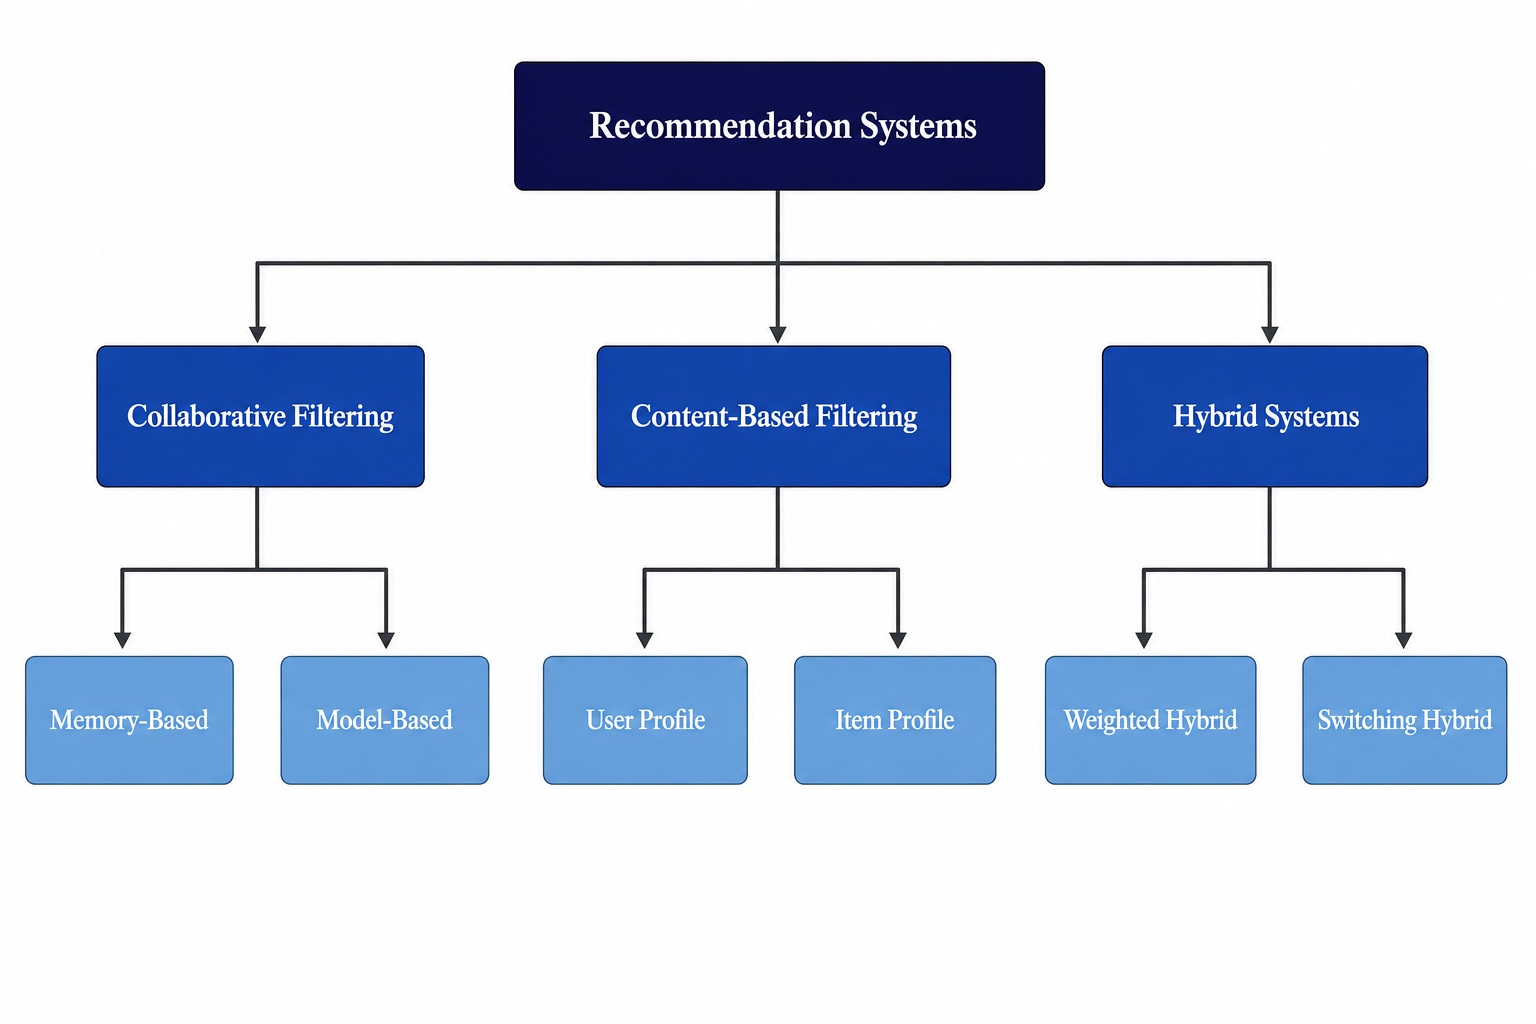
\includegraphics[width=0.95\textwidth]{picture/figures/schemas/taxonomy_reco.png}
    \caption{Taxonomy of Recommendation System Types.}
    \label{fig:rs_taxonomy}
\end{figure}

Out of the above, sequential recommendation systems form a subcategory and have
gradually become a more and more important area of collaborative filtering,
where the order in which users interacted with items is considered. This work
concentrates only on this type of systems. Formally they are defined below.

\section{Sequential Recommendation}

In sequential recommendation (SR), the task of predicting the next item to recommend to a user depends not only on the set of items with which the user has interacted, but also on the specific order of these interactions \citep{pan2024survey}. This sequence is important, as users' preferences are dynamic: short-term preferences often have higher weight than long-term ones and the meaning of the action is interpreted differently based on the context that precedes it (for example, clicking an item does not carry the same semantics as purchasing it). SR is typically framed as the task of predicting the next item given a sequence of past interactions and is naturally suited for scenarios where dynamic, short-term intent needs to be modeled, such as e-commerce, news recommendation, or media streaming \citep{hidasi2016gru4rec,kang2018sasrec,sun2019bert4rec}.

Deep learning has led to major advances in the area of SR, due to models that are able to incorporate sequential dependencies explicitly. Among the early ones, the use of gated recurrent networks such as GRU4Rec was shown to be effective in capturing session-level dynamics and improving next-item prediction \citep{hidasi2016gru4rec}. Self-attention based models, like SASRec, proposed an effective solution to capture long-range dependencies \citep{kang2018sasrec}, and then BERT4Rec utilized bidirectional context through a masked item prediction objective \citep{sun2019bert4rec}. These papers have consolidated SR as a major research direction in recommender systems.

In practice, SR remains challenging because interaction sequences can be very sparse, short, long, or heterogeneous, which complicates accurate modeling. Short sequences contain little evidence about user preferences, while long sequences may include irrelevant interactions that dilute the user's current intent. Moreover, variable time gaps between interactions and differing action semantics increase the difficulty of balancing short-term and long-term interests. Consequently, recent work emphasizes more powerful sequence encoders, hybrid architectures that combine global and local signals, incorporation of side information, and integration with large language models to improve robustness and representation quality \citep{pan2024survey}.

\begin{figure}[htbp]
    \centering
    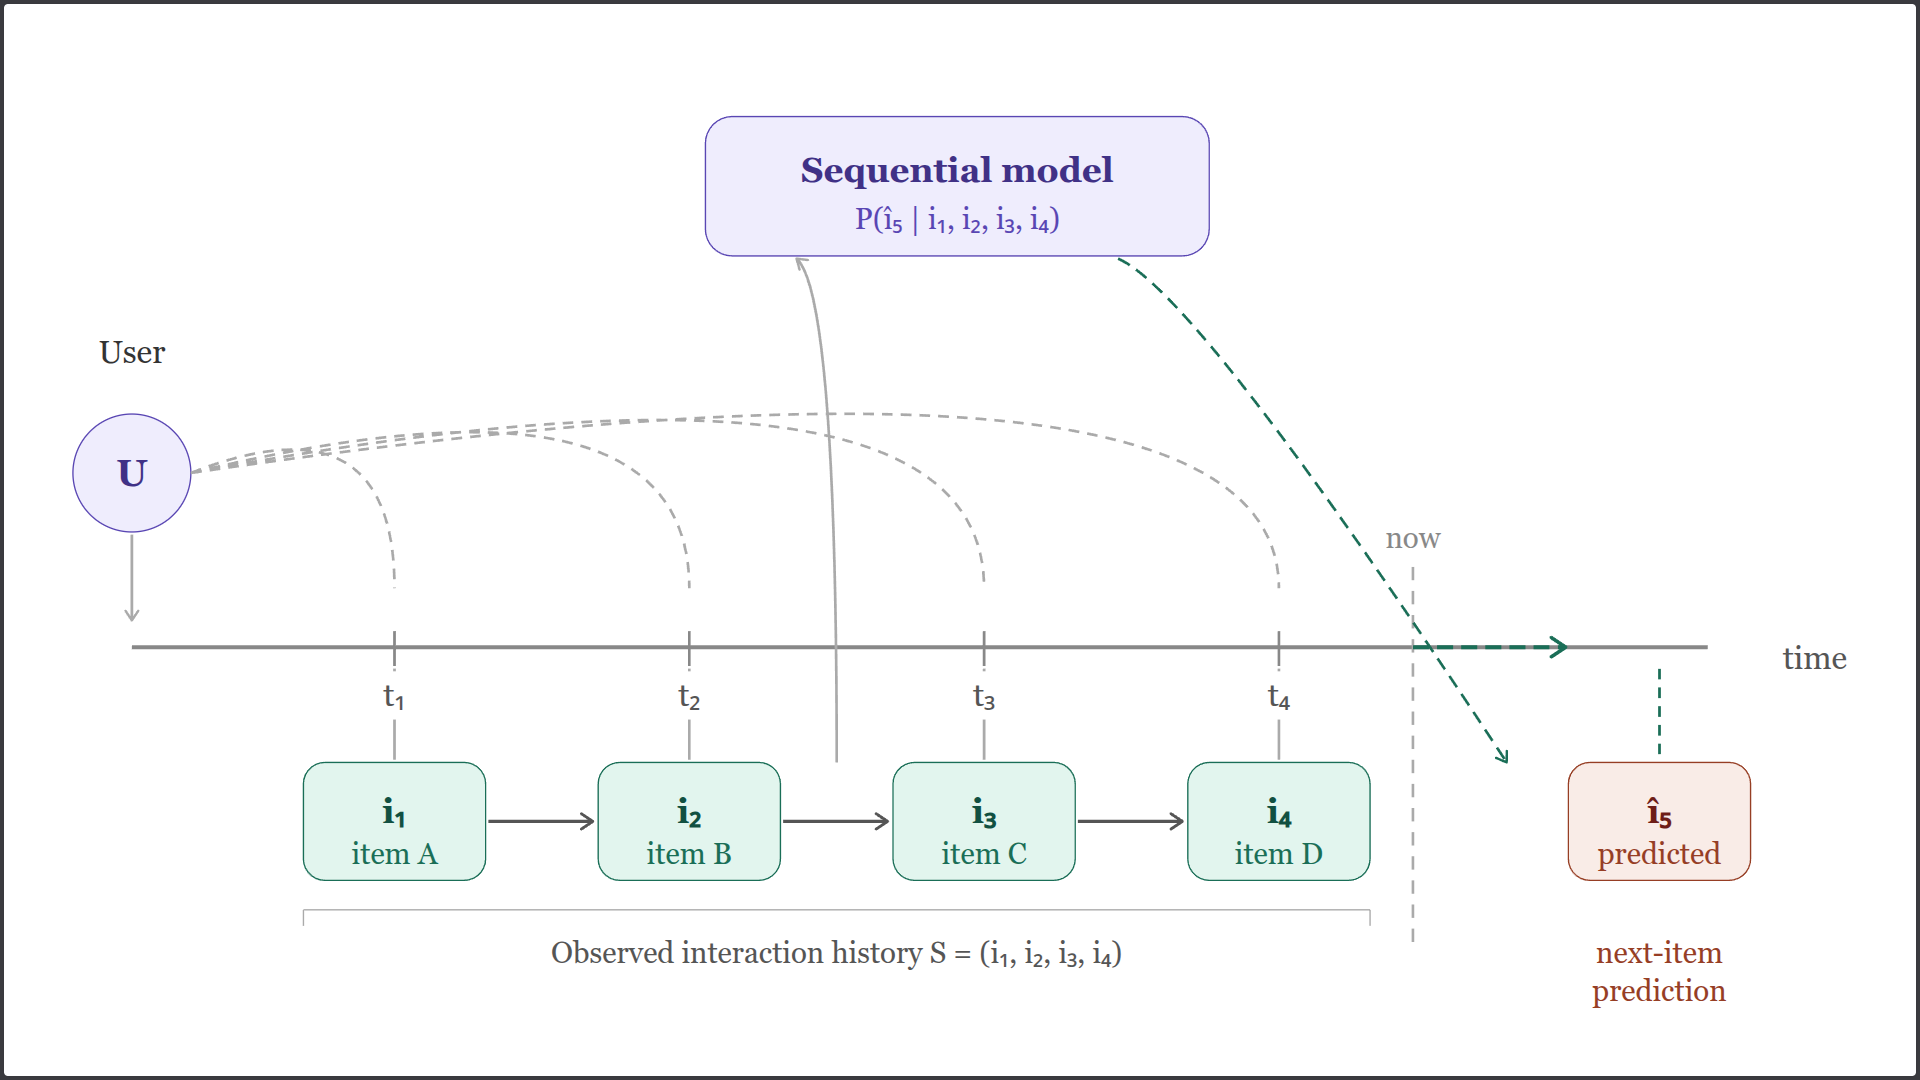
\includegraphics[
        width=0.9\textwidth,
        trim=20 20 20 20,
        clip
    ]{picture/figures/schemas/sequential_recommendation_timeline.png}
    \caption{Illustration of a user interaction timeline for next-item prediction.}
    \label{fig:sequential_timeline}
\end{figure}

\section{Sequence-Based Models}

Sequence-based models constitute an important class of sequential recommendation
methods that explicitly exploit the ordered nature of user interaction histories.
Unlike simpler approaches that treat a user's past actions as an unordered set,
these models learn patterns from the exact sequence of events in order to
predict the next likely item. This family of methods formed one of the earliest
and most influential directions in sequential recommendation, and it includes
recurrent, convolutional, and Transformer-based architectures.

\subsection{GRU4Rec}

GRU4Rec was one of the first deep learning models proposed for session-based
recommendation and showed that recurrent neural networks can effectively model
sequential user behavior \citep{hidasi2016gru4rec}. The model uses gated
recurrent units to process interaction sequences in order, allowing it to
capture short-term dependencies and session-level dynamics. Its key idea is that
the hidden state summarizes the recent behavior of the user, which is then used
to predict the next item in the sequence. This made GRU4Rec an important
baseline for later sequential recommendation research.

\subsection{Caser}

Caser introduces a convolutional approach to sequential recommendation by
embedding a user's recent interaction history into a two-dimensional
representation and applying convolutional filters over it \citep{tang2018caser}.
The model is designed to capture both general user preferences and local
sequential patterns through vertical and horizontal convolutions. In contrast to
recurrent models, Caser views the sequence as a structured pattern detection
problem, which allows it to learn influential subsequences and short-range
dependencies. This makes Caser a representative CNN-based baseline in the SR
literature.

\subsection{SASRec}

SASRec applies self-attention to sequential recommendation, using a
Transformer-style architecture to model long-range dependencies between
interacted items \citep{kang2018sasrec}. Instead of processing the sequence
strictly step by step, the model learns which past items are most relevant to
the current prediction through attention weights. This gives SASRec a strong
ability to capture both short- and long-term behavioral patterns while remaining
efficient to train. It became one of the most influential Transformer-based
baselines in sequential recommendation.

\subsection{BERT4Rec}

BERT4Rec extends the Transformer idea by adopting a bidirectional encoding
strategy and a masked item prediction objective \citep{sun2019bert4rec}. Rather
than predicting the next item in a strictly left-to-right fashion, the model
randomly masks items in the sequence and learns to reconstruct them from both
left and right context. This training objective encourages richer sequence
representations and often improves the quality of learned user behavior
embeddings. BERT4Rec is widely used as a strong benchmark for sequential
recommendation due to its ability to model contextual dependencies more deeply.

\begin{figure}[htbp]
    \centering
    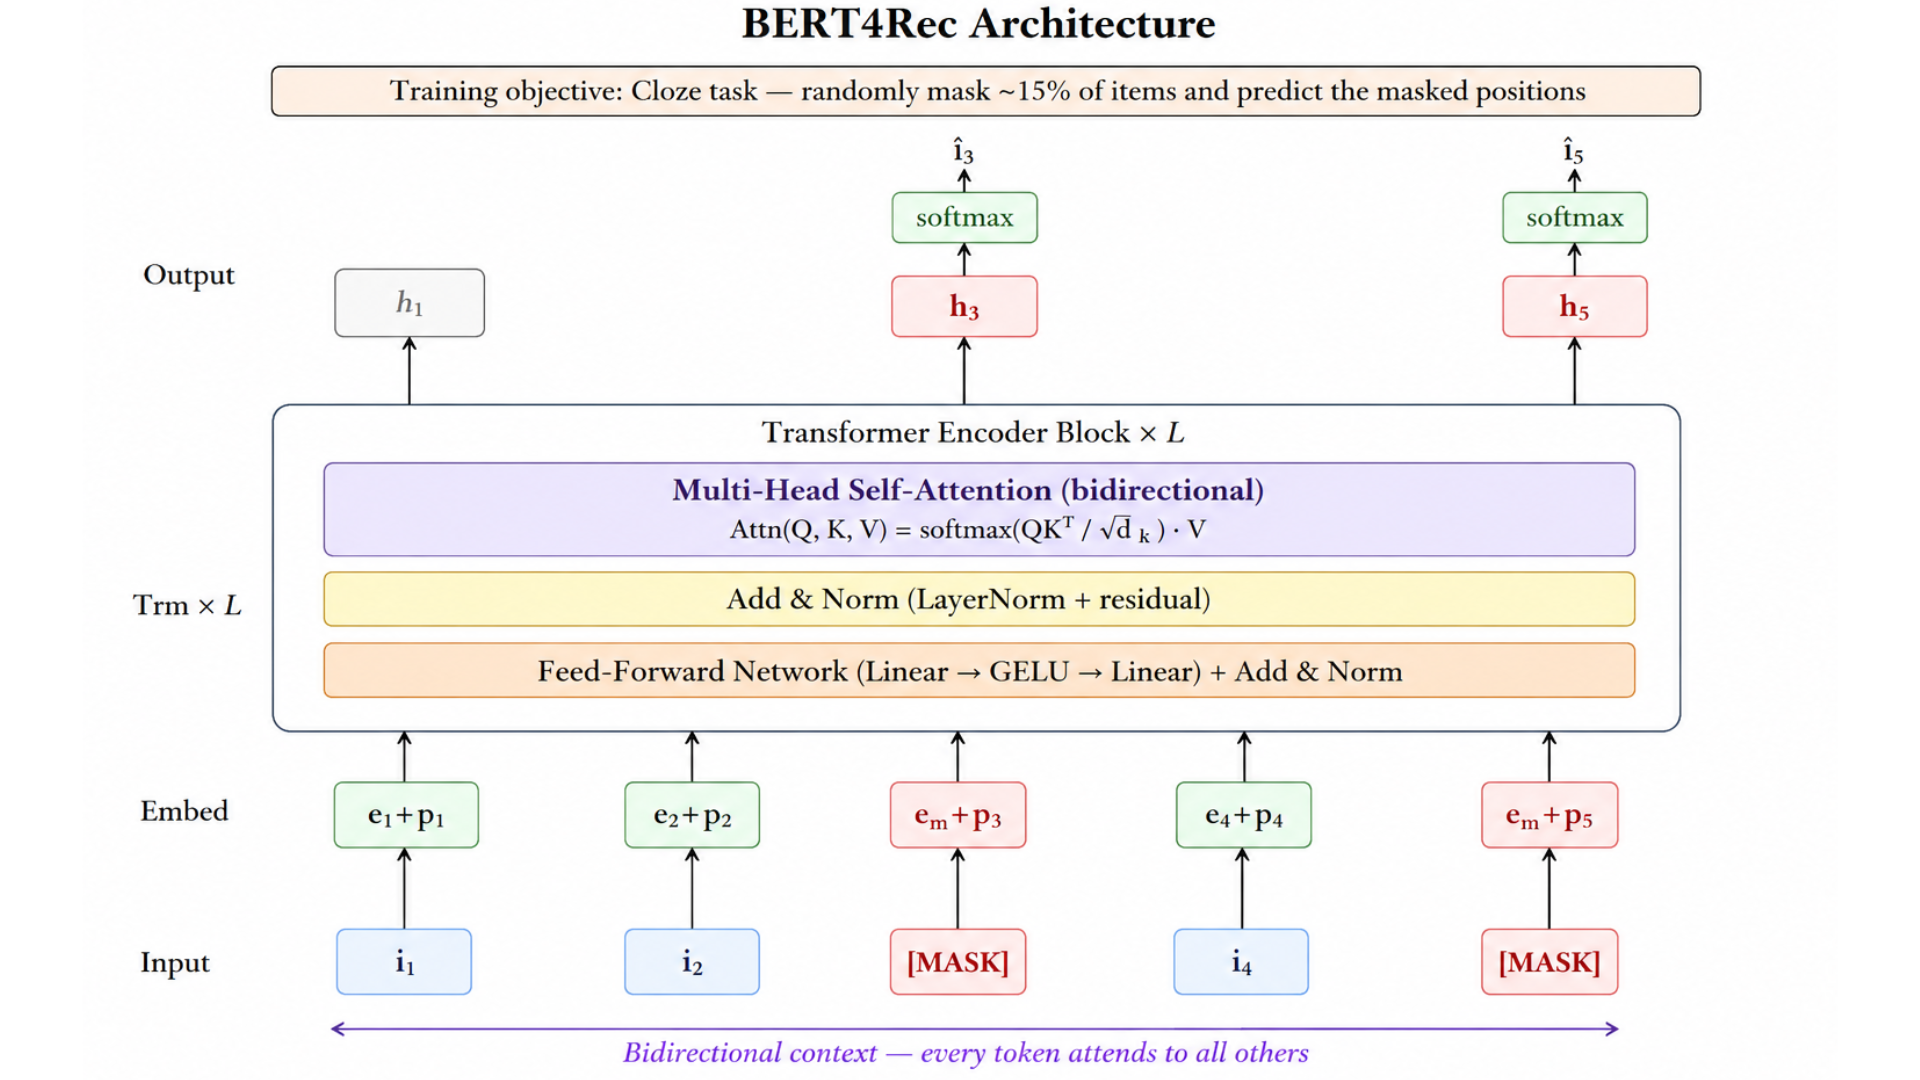
\includegraphics[width=0.9\textwidth]{picture/figures/schemas/bert4rec_architecture.png}
    \caption{Architecture illustration of a sequence-based model such as SASRec or BERT4Rec.}
    \label{fig:sequence_architecture}
\end{figure}

\begin{table}[h]
\centering
\begin{tabular}{p{2.4cm} p{3.3cm} p{7.0cm}}
\toprule
\textbf{Model} & \textbf{Approach} & \textbf{Key idea} \\
\midrule
GRU4Rec & Recurrent neural network & Models the interaction sequence step by step with gated recurrent units. \\
Caser & Convolutional neural network & Learns local sequential patterns from a sequence-as-image representation. \\
SASRec & Self-attention / Transformer encoder & Uses attention to focus on the most relevant past items for next-item prediction. \\
BERT4Rec & Bidirectional Transformer encoder & Learns contextual sequence representations using masked item prediction. \\
\bottomrule
\end{tabular}
\caption{Representative sequence-based recommendation models.}
\label{tab:sequence_models}
\end{table}

\section{Graph-Based Models / GNN}

Graph-based recommender systems model user-item interactions as a graph, where
users and items are represented as nodes and historical interactions are encoded
as edges. This formulation is useful because recommendation data are naturally
relational: a user's preference can be inferred not only from their own history,
but also from their position in the interaction graph and from the neighborhoods
of connected users and items. Graph neural networks therefore provide a powerful
way to propagate collaborative signals, capture higher-order connectivity, and
learn richer embeddings than methods based solely on local sequence patterns
\citep{wu2020gnnsurvey,he2020lightgcn}.

\subsection{LightGCN}

LightGCN is one of the most influential graph-based recommendation models
because it simplifies graph convolution to its essential component:
neighborhood aggregation \citep{he2020lightgcn}. Instead of using feature
transformation and nonlinear activation, LightGCN directly propagates user and
item embeddings over the bipartite interaction graph and combines the embeddings
from multiple propagation layers to obtain the final representation. This makes
the model both efficient and effective, and it has become a standard baseline
for graph-based collaborative filtering. Its main strength is the ability to
capture collaborative signals from the full interaction graph while remaining
simple enough to train and interpret.

\begin{table}[h]
\centering
\begin{tabular}{p{3cm} p{3cm} p{6.8cm}}
\toprule
\textbf{Model} & \textbf{Approach} & \textbf{Key idea} \\
\midrule
LightGCN & Graph collaborative filtering & Learns user and item embeddings by propagating them over the bipartite interaction graph with only neighborhood aggregation. \\
\bottomrule
\end{tabular}
\caption{Representative graph-based recommendation models.}
\label{tab:graph_models}
\end{table}

\begin{figure}[htbp]
    \centering
    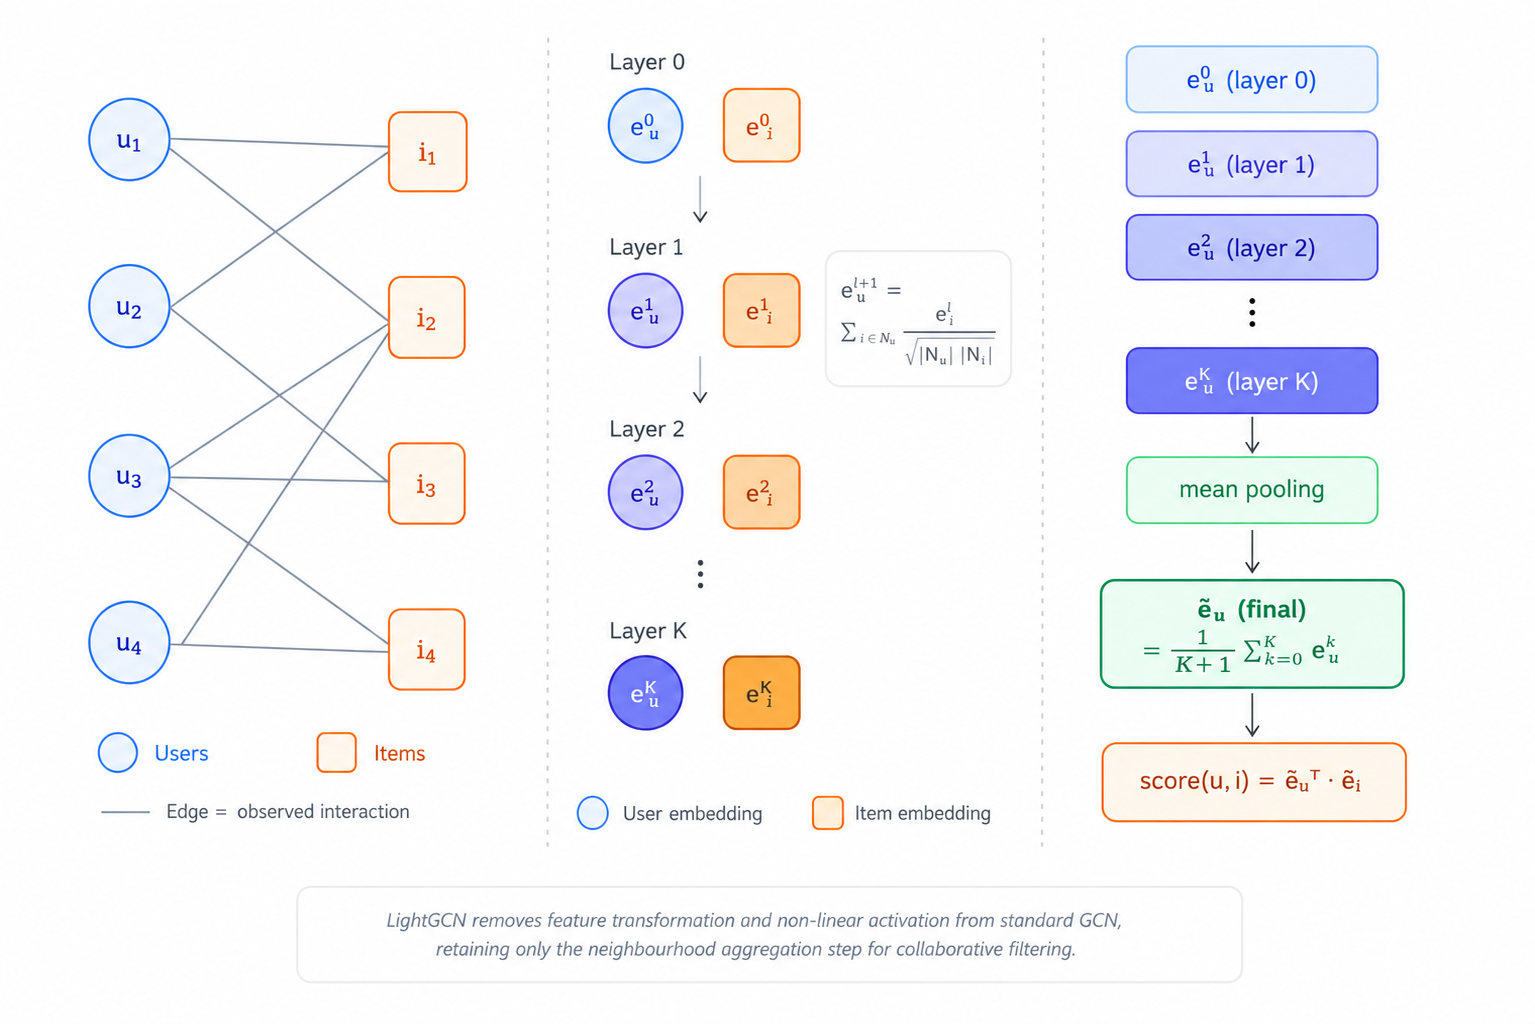
\includegraphics[width=0.9\textwidth]{picture/figures/schemas/lightgcn_bipartite_graph.png}
    \caption{Illustration of a user-item bipartite graph and embedding propagation in LightGCN.}
    \label{fig:lightgcn_graph}
\end{figure}

\section{LLMs Applied to Sequential Recommendation}

Large Language Models (LLMs) have recently entered recommendation systems by
bringing strong semantic understanding of text, contextual reasoning, and
transferable representations learned from large-scale corpora. In sequential
recommendation, this is particularly valuable because many items are described
by textual metadata such as titles, descriptions, reviews, or categorical
attributes. Rather than relying only on item identifiers or interaction history,
LLM-based methods can transform item text into dense embeddings that encode
semantic similarity and can be injected into recommendation pipelines as
initialization, side information, or direct ranking signals
\citep{harte2023leveraging,llmrec2024,wu2023survey,liu2024llmers}.

A central idea in this line of work is that the textual description of an item
can act as a semantic bridge between sparse interaction data and richer domain
knowledge. When item descriptions are encoded by an LLM, the resulting
embeddings can capture not only surface-level wording, but also relations
between concepts, product properties, and user-facing meaning. These embeddings
can then be used to improve sequential recommenders by initializing item
representations, enhancing content-based signals, or supporting hybrid models
that combine textual and behavioral information. This is especially helpful in
cold-start or sparse-data settings, where item IDs alone provide little
information about the item's semantics.

\begin{figure}[htbp]
    \centering
    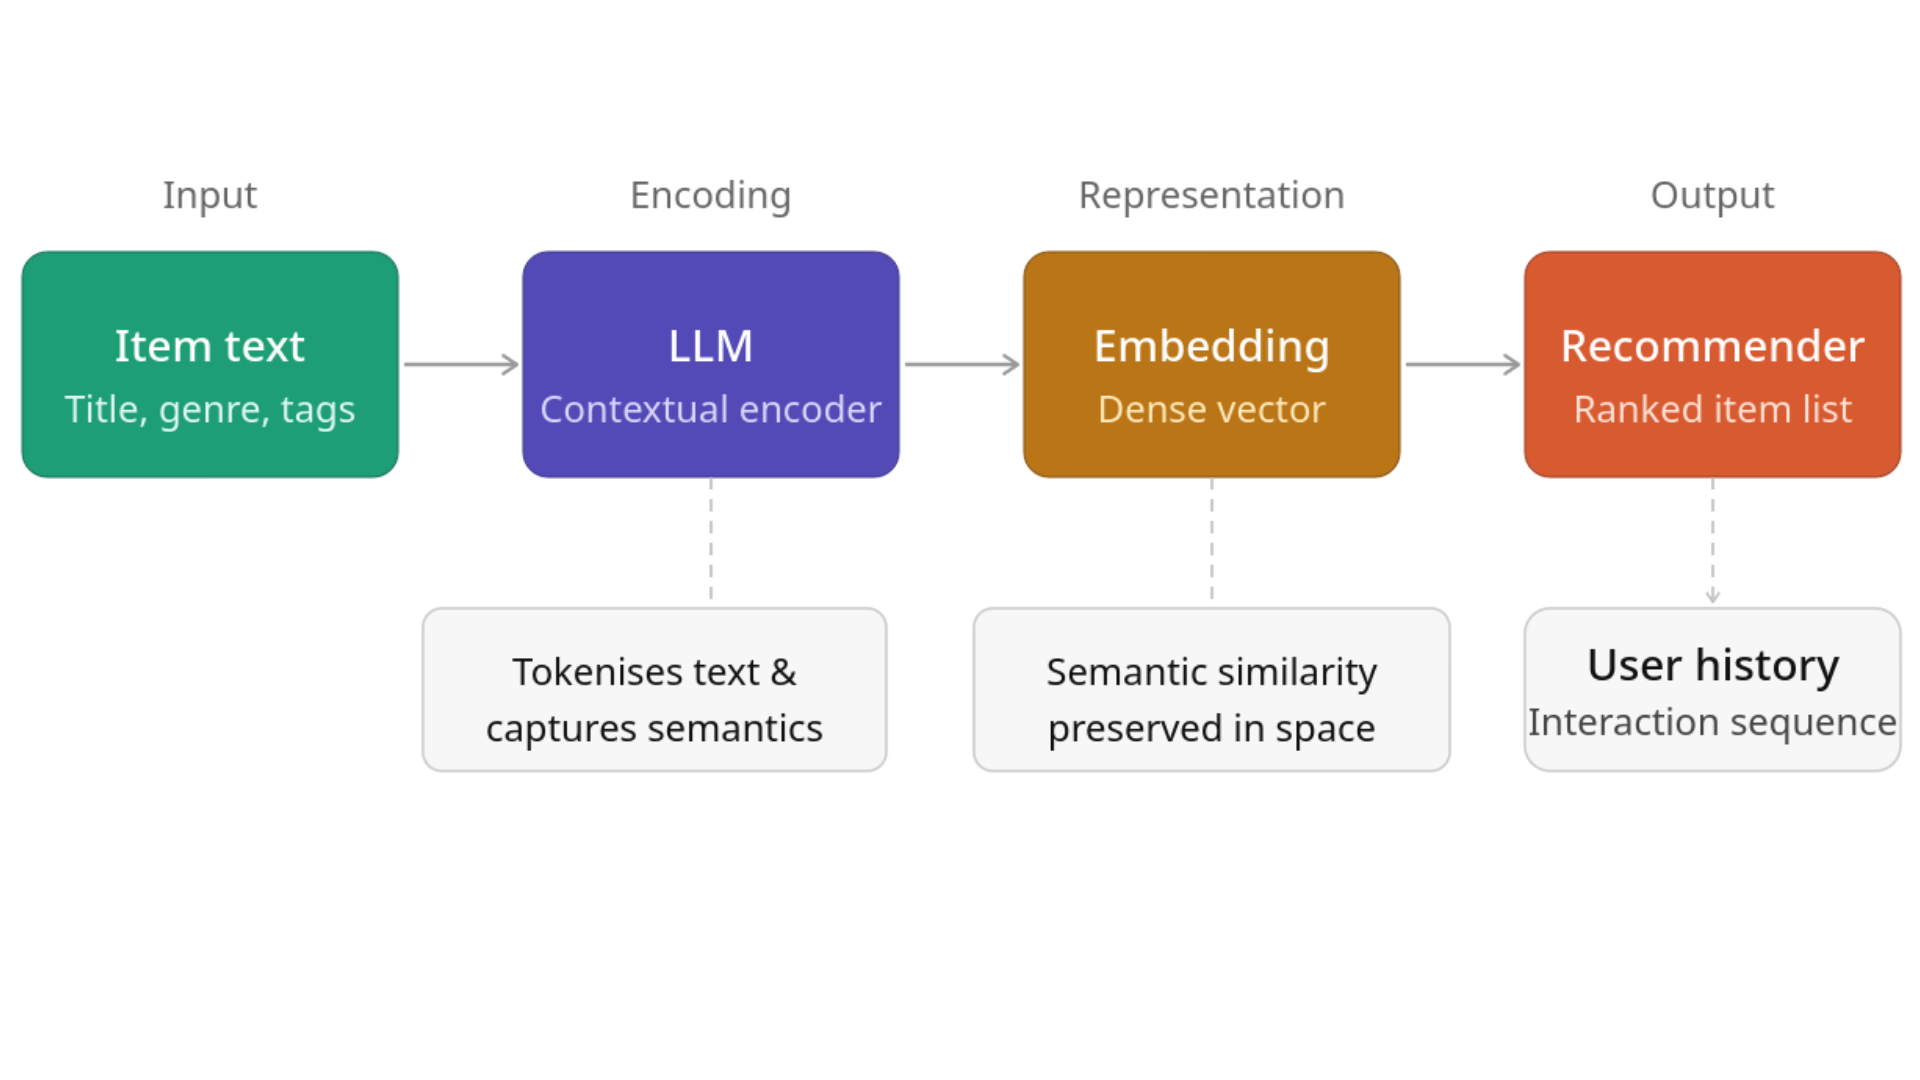
\includegraphics[width=0.92\textwidth]{picture/figures/schemas/llm_pipeline.png}
    \caption{Pipeline for using item descriptions to generate embeddings with an LLM and feed them into a recommender.}
    \label{fig:llm_pipeline}
\end{figure}

Recent studies have shown that LLMs can be used in several ways for sequential
recommendation. Some approaches initialize strong sequential models such as
BERT4Rec or SASRec with LLM-derived embeddings, while others fine-tune the LLM
directly for recommendation or use it as a semantic encoder for items and user
profiles \citep{harte2023leveraging,llmrec2024,wu2023survey}. Survey work also
highlights a broader shift from treating LLMs only as feature extractors toward
using them as integrated components of recommendation pipelines, including
knowledge enhancement, interaction enhancement, and model enhancement
\citep{liu2024llmers}. This makes LLMs a promising direction for improving both
representation quality and generalization in sequential recommendation.

At the same time, the usefulness of LLMs depends strongly on how item text is
constructed and presented. A short product title, a structured attribute list,
and a longer user-centric description can lead to different embedding spaces and
therefore different recommendation behaviors. For this reason, item text
design is not a trivial preprocessing step, but an important modeling choice
that can influence semantic richness, distinctiveness, and downstream
performance. This observation motivates the empirical study carried out in this
memoir, where different item description strategies are analyzed in the context
of sequential recommendation.

\begin{table}[h]
\centering
\begin{tabular}{p{3cm} p{3.5cm} p{6.3cm}}
\toprule
\textbf{Use case} & \textbf{Method} & \textbf{Key idea} \\
\midrule
Embedding initialization & LLM $\rightarrow$ item vectors & Use semantic embeddings to initialize or enrich sequential recommenders. \\
Direct recommendation & LLM as recommender & Fine-tune or prompt the LLM to rank candidate items directly. \\
Hybrid enhancement & LLM + sequential model & Combine textual embeddings with behavioral sequence modeling. \\
\bottomrule
\end{tabular}

\caption{Examples of how LLMs are used in sequential recommendation.}
\label{tab:llm_seq}
\end{table}


\section{Evaluation Metrics}

To evaluate the performance of sequential recommendation models, this memoir
uses three standard ranking-based metrics: Hit Ratio at \(K\) (HR@K),
Normalized Discounted Cumulative Gain at \(K\) (NDCG@K), and Mean Reciprocal
Rank (MRR). These metrics measure how well the model places the true next item
among its top-ranked predictions. Since sequential recommendation is typically a
top-\(K\) ranking problem, such metrics are more informative than simple
classification accuracy.

\subsection{Hit Ratio at \(K\)}

HR@K measures whether the ground-truth next item appears in the top-\(K\)
recommended items. It gives a binary reward of 1 if the target item is present
in the recommendation list and 0 otherwise. As a result, HR@K captures the
model's ability to retrieve the correct item within a limited number of
suggestions, but it does not consider the exact rank position inside the top-\(K\).

\subsection{Normalized Discounted Cumulative Gain at \(K\)}

NDCG@K evaluates both whether the correct item is retrieved and how high it is
ranked in the recommendation list. Higher-ranked correct predictions receive
larger scores, which makes NDCG@K more sensitive to the ordering quality of the
top-\(K\) list. This metric is especially useful when the position of the
predicted item matters, which is often the case in practical recommendation
scenarios.

\subsection{Mean Reciprocal Rank}

MRR measures the inverse of the rank position of the first relevant item.
Unlike HR@K, it rewards models that place the target item very close to the top
of the list. If the correct item is ranked first, the reciprocal rank is 1; if
it is ranked second, it is \(1/2\), and so on. MRR therefore reflects how early
the desired item appears in the ranked output.

\begin{table}[h]
\centering
\begin{tabular}{p{2.5cm} p{5.2cm} p{5.5cm}}
\toprule
\textbf{Metric} & \textbf{Formula} & \textbf{What it measures} \\
\midrule
HR@K &
\[
\mathrm{HR@K} = \frac{1}{N}\sum_{i=1}^{N}\mathbb{I}(\text{rank}_i \leq K)
\]
&
Whether the true next item appears in the top-\(K\) recommendations. \\
\midrule
NDCG@K &
\[
\mathrm{NDCG@K} = \frac{1}{N}\sum_{i=1}^{N}\frac{\mathbb{I}(\text{rank}_i \leq K)}{\log_2(\text{rank}_i + 1)}
\]
&
Retrieval quality with a stronger reward for higher-ranked correct items. \\
\midrule
MRR &
\[
\mathrm{MRR} = \frac{1}{N}\sum_{i=1}^{N}\frac{1}{\text{rank}_i}
\]
&
How early the first relevant item appears in the ranked list. \\
\bottomrule
\end{tabular}
\caption{Ranking Metrics for Sequential Recommendation.}
\label{tab:evaluation_metrics}
\end{table}

\section{Conclusion}

This chapter introduced the fundamental concepts underlying recommendation
systems and provided an overview of the main paradigms used in practice,
including collaborative filtering, sequence-based models, graph-based models,
and LLM-enhanced approaches. It also presented the sequential recommendation
setting, the principal baseline architectures used in this work, and the
evaluation metrics employed to assess model performance.

Despite the progress made by these methods, several limitations remain,
particularly in the way they model heterogeneous user histories, combine
global and local signals, and exploit textual item information. These open
questions motivate the research gaps addressed in the following chapter.


\section{Identified Gaps and Positioning of Contributions}

Despite the substantial progress achieved by recent sequential recommendation
methods, two important gaps remain insufficiently addressed in the literature.
First, many hybrid GNN-Transformer approaches combine global graph signals and
local sequential signals using a fixed or uniform fusion strategy, without
considering that users exhibit different interaction history profiles. In
practice, users with sparse histories benefit more from global collaborative
information, whereas users with rich histories can better exploit detailed
sequential patterns. This observation motivates our first contribution, which
introduces a length-adaptive fusion mechanism that dynamically balances graph-
based and sequence-based representations according to the amount of available
user history.

Second, although large language models have recently been integrated into
recommendation systems, the influence of item textual description strategy on
the quality of the resulting embeddings has not yet been systematically
explored. Different forms of item text, such as titles, structured attributes,
or user-oriented descriptions, may produce embeddings with different semantic
properties and downstream effects on recommendation performance. This gap
motivates our second contribution, which conducts a systematic study of how item
description design affects LLM embeddings in sequential recommendation.

Together, these two gaps define the positioning of this memoir: the first
contribution addresses the adaptive fusion of structural and sequential signals,
while the second investigates the semantic role of item text in LLM-based
sequential recommendation.

% ============================================================
%  CHAPTER 2 — Length-Adaptive Hybrid GNN-Transformer
% ============================================================
\chapter{Length-Adaptive Hybrid GNN-Transformer for Sequential Recommendation}

\section{Introduction}

Sequential recommendation remains a challenging problem because user interaction
histories are heterogeneous in both length and density. Transformer-based models
such as SASRec \citep{kang2018sasrec} and BERT4Rec \citep{sun2019bert4rec} have
demonstrated strong performance by capturing long-range dependencies within
interaction sequences, but they rely on the availability of sufficiently long
histories to generalize reliably. Graph Neural Network models such as LightGCN
\citep{he2020lightgcn} address this by aggregating global collaborative signals
from the full user-item interaction graph, making them more robust for sparse
users. However, when used in isolation, each paradigm captures only one side of
the recommendation signal: sequence models ignore global item co-occurrence
structure, while graph models ignore the fine-grained temporal order of
individual user interactions \citep{wu2020gnnsurvey, pan2024survey}.

This chapter proposes a Length-Adaptive Hybrid GNN-Transformer, a model that
combines both paradigms through a user-specific fusion mechanism controlled by
the length of each user's interaction history. The core idea is that the
relative reliability of the graph signal versus the sequence signal is not
constant across users: it varies directly with the amount of available
sequential evidence. The proposed model quantifies this variation through a
scalar weight \(\lambda(u)\) that dynamically adjusts the contribution of the
GNN and Transformer branches for each user individually. The remainder of this
chapter is organized as follows: Section~\ref{sec:limitations} discusses the
limitations of existing models and formally states the research problem;
Section~\ref{sec:solution} introduces the adaptive fusion mechanism and the
formal problem definition; Section~\ref{sec:family} presents the family of
hybrid model variants; and Section~\ref{sec:ch2conclusion} concludes the
chapter.


\section{Limitations of Existing Models and Problem Statement}
\label{sec:limitations}

Despite the progress achieved by the models reviewed in Chapter~1, three
concrete limitations can be identified in the existing literature on hybrid
GNN-Transformer sequential recommendation.

\textbf{Limitation 1 --- Fixed fusion weights in existing hybrid models.}
Hybrid approaches that combine GNN and Transformer components, such as those
surveyed in \citep{wu2020gnnsurvey}, typically apply a single global fusion
weight that is shared uniformly across all users. This fixed weighting strategy
treats every user identically, regardless of how much interaction history is
available. As a result, the model cannot adapt to the fact that the relative
informativeness of the graph signal versus the sequence signal varies
substantially from one user to another. A fixed weight that is optimal on
average will systematically underserve both sparse users and dense users
\citep{pan2024survey}.

\textbf{Limitation 2 --- Transformer-only models fail sparse users.}
Self-attention mechanisms, as used in SASRec \citep{kang2018sasrec} and
BERT4Rec \citep{sun2019bert4rec}, require a sufficient number of interactions
to produce reliable contextualized representations. When a user has only a
small number of past interactions, the self-attention layers lack enough context
to generalize, and the resulting sequence embedding is noisy or
underspecified. These models therefore provide poor recommendations for sparse
and cold-start users, a critical segment in any real-world recommendation
platform.

\textbf{Limitation 3 --- GNN-only models waste dense users' sequential patterns.}
Graph-based models such as LightGCN \citep{he2020lightgcn} aggregate
neighborhood information over the full interaction graph and produce strong
collaborative embeddings for sparse users. However, they do not model the
temporal order of a user's individual interactions. For users with long, rich
interaction histories, this means that fine-grained sequential patterns ---
the exact order in which items were consumed, recency effects, and evolving
preferences --- are entirely discarded. The graph signal alone is insufficient
to capture dynamic intent for active users \citep{pan2024survey}.

\begin{figure}[htbp]
    \centering
    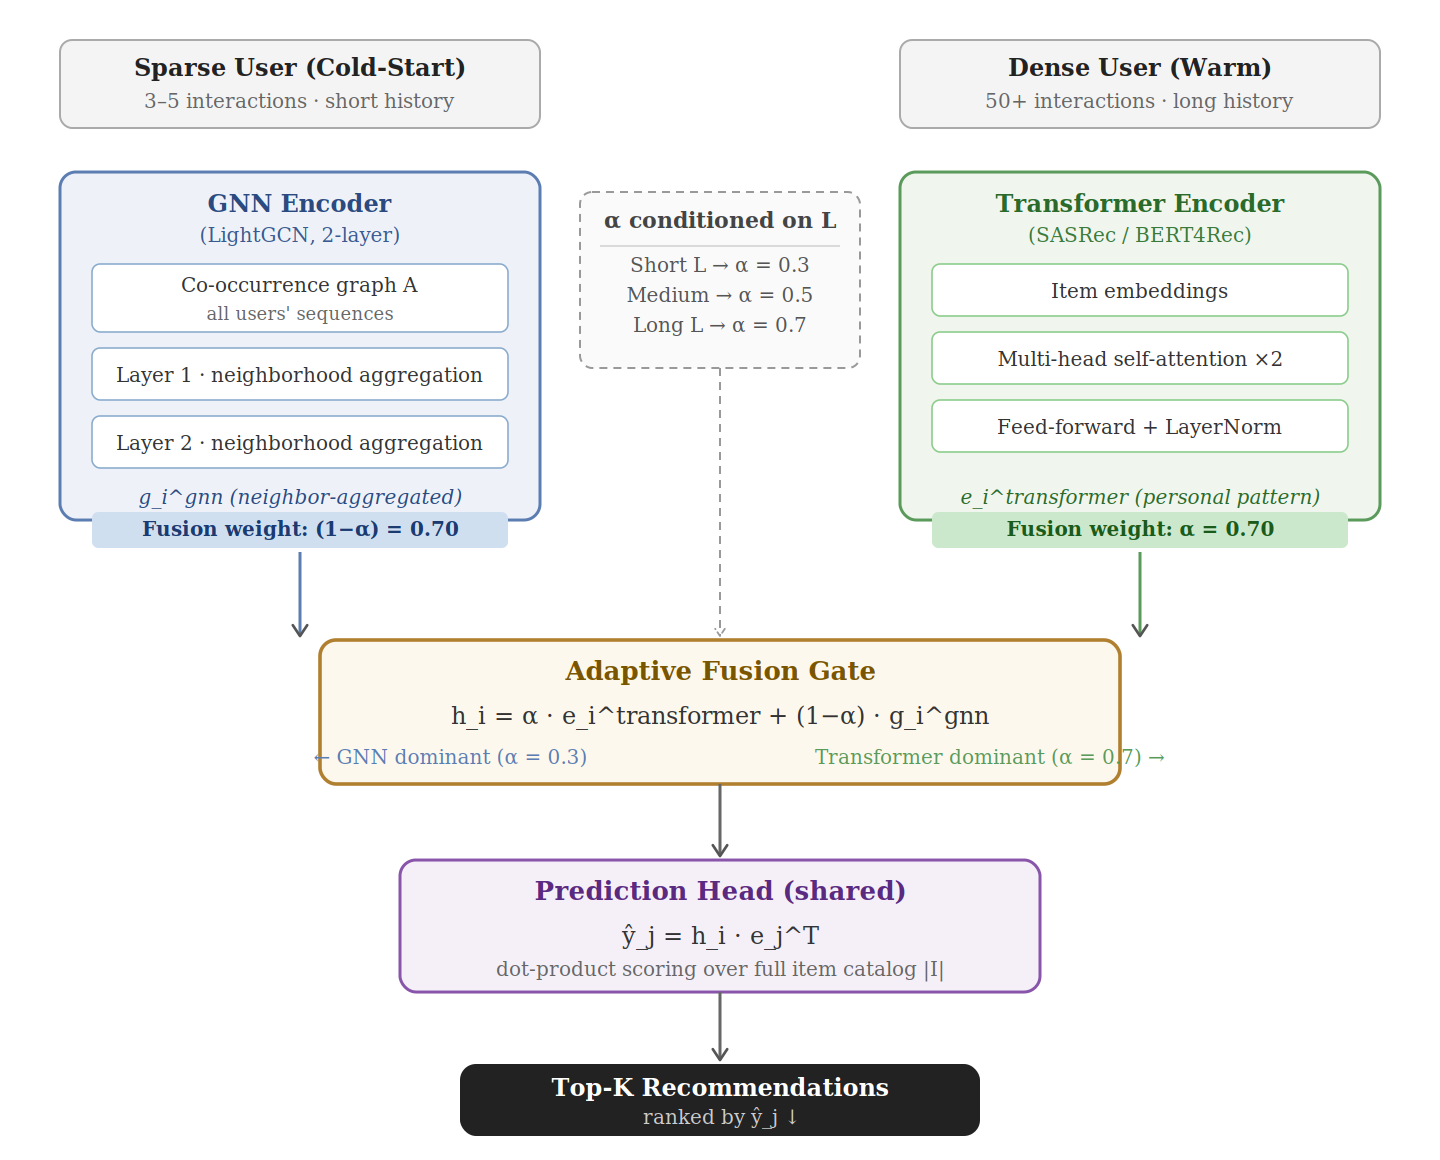
\includegraphics[width=0.9\textwidth]{picture/figures/schemas/sparse_dense_comparison.png}
    \caption{Comparison of sparse and dense user history profiles and their
    ideal information source: sparse users benefit from global GNN signals,
    while dense users benefit from fine-grained Transformer sequential modeling.}
    \label{fig:sparse_dense}
\end{figure}

\subsection*{Problem Statement}

The three limitations above converge on a single fundamental question, which
constitutes the first research problematic of this memoir:

\begin{mdframed}[
    linecolor=black, linewidth=0.8pt,
    innertopmargin=10pt, innerbottommargin=10pt,
    innerleftmargin=14pt, innerrightmargin=14pt,
    roundcorner=3pt
]
\textit{How to dynamically adapt the fusion between global graph signals and
local sequential modelling according to each user's interaction history
profile?}
\end{mdframed}

Answering this question requires a model that is aware of each user's
interaction density and uses this information to balance the GNN and
Transformer contributions at the individual user level, rather than applying
a fixed global weight. This is the design principle that motivates the
proposed architecture described in the following section.


\section{Proposed Solution: The Adaptive Fusion Mechanism}
\label{sec:solution}

\subsection{Formal Problem Definition}

Let \(\mathcal{U}\) and \(\mathcal{I}\) denote the sets of users and items,
respectively. For each user \(u \in \mathcal{U}\), let
\(S_u = (i_1, i_2, \ldots, i_{n_u})\) be their interaction history of length
\(n_u\), where each \(i_t \in \mathcal{I}\) is an item consumed at time step
\(t\), ordered chronologically. The task of next-item sequential recommendation
is defined as: given the prefix \(S_u^{(t)} = (i_1, \ldots, i_t)\), learn a
scoring function

\begin{equation}
    f_{\Theta}\!\left(u,\, S_u^{(t)},\, j\right) \in \mathbb{R}
    \label{eq:scoring}
\end{equation}

\noindent that assigns a relevance score to each candidate item
\(j \in \mathcal{I}\), where \(\Theta\) denotes all trainable parameters. At
inference time, items are ranked by their scores and top-\(K\) accuracy is
evaluated via HR@\(K\), NDCG@\(K\), and MRR@\(K\) as defined in
Chapter~1.

\subsection{The Adaptive Fusion Mechanism}

The proposed model computes two independent representations for each user
\(u\): a graph-based representation \(\mathbf{h}_u^{\text{GNN}}\), produced by
a Graph Neural Network encoder operating over the global item co-occurrence
graph, and a sequence-based representation \(\mathbf{h}_u^{\text{Trans}}\),
produced by a Transformer encoder operating over the user's personal
interaction history \(S_u\). These two representations are then combined
through a user-specific scalar weight \(\lambda(u) \in [0, 1]\):

\begin{equation}
    \mathbf{h}_u = \lambda(u)\cdot \mathbf{h}_u^{\text{Trans}}
    + \bigl(1 - \lambda(u)\bigr)\cdot \mathbf{h}_u^{\text{GNN}}
    \label{eq:fusion}
\end{equation}

\noindent where the fusion weight \(\lambda(u)\) is derived from the user's
interaction history length \(n_u\) and a normalization factor \(n_{\max}\),
the maximum history length observed in the training set:

\begin{equation}
    \lambda(u) = \sigma\!\left(\frac{n_u}{n_{\max}}\right)
    \label{eq:lambda}
\end{equation}

\noindent and \(\sigma(\cdot)\) denotes the sigmoid function
\(\sigma(x) = 1/(1 + e^{-x})\).

\subsection{Intuition and Rationale}

The intuition behind Equations~\ref{eq:fusion} and~\ref{eq:lambda} is
straightforward. When a user has a short interaction history (\(n_u\) is
small), \(\lambda(u)\) is close to 0, and the fused representation
\(\mathbf{h}_u\) relies predominantly on \(\mathbf{h}_u^{\text{GNN}}\). This
is desirable because the GNN aggregates global co-occurrence signals from all
users in the training set and is therefore informative even when individual
sequence evidence is scarce. Conversely, when a user has a long interaction
history (\(n_u\) is large), \(\lambda(u)\) approaches 1, and \(\mathbf{h}_u\)
relies predominantly on \(\mathbf{h}_u^{\text{Trans}}\). In this regime, the
Transformer can exploit the full richness of the user's personal sequential
patterns, which carry more information than global averages.

The use of history length \(n_u\) as the proxy variable is motivated by the
observation that the reliability of self-attention degrades when the input
sequence is too short \citep{kang2018sasrec, sun2019bert4rec}, while GNN
neighborhood aggregation is length-independent by construction
\citep{he2020lightgcn}. The sigmoid normalization in
Equation~\ref{eq:lambda} ensures that \(\lambda(u)\) remains bounded in
\([0, 1]\) and transitions smoothly between the two extremes, avoiding hard
discontinuities in the embedding space.

\begin{figure}[htbp]
    \centering
    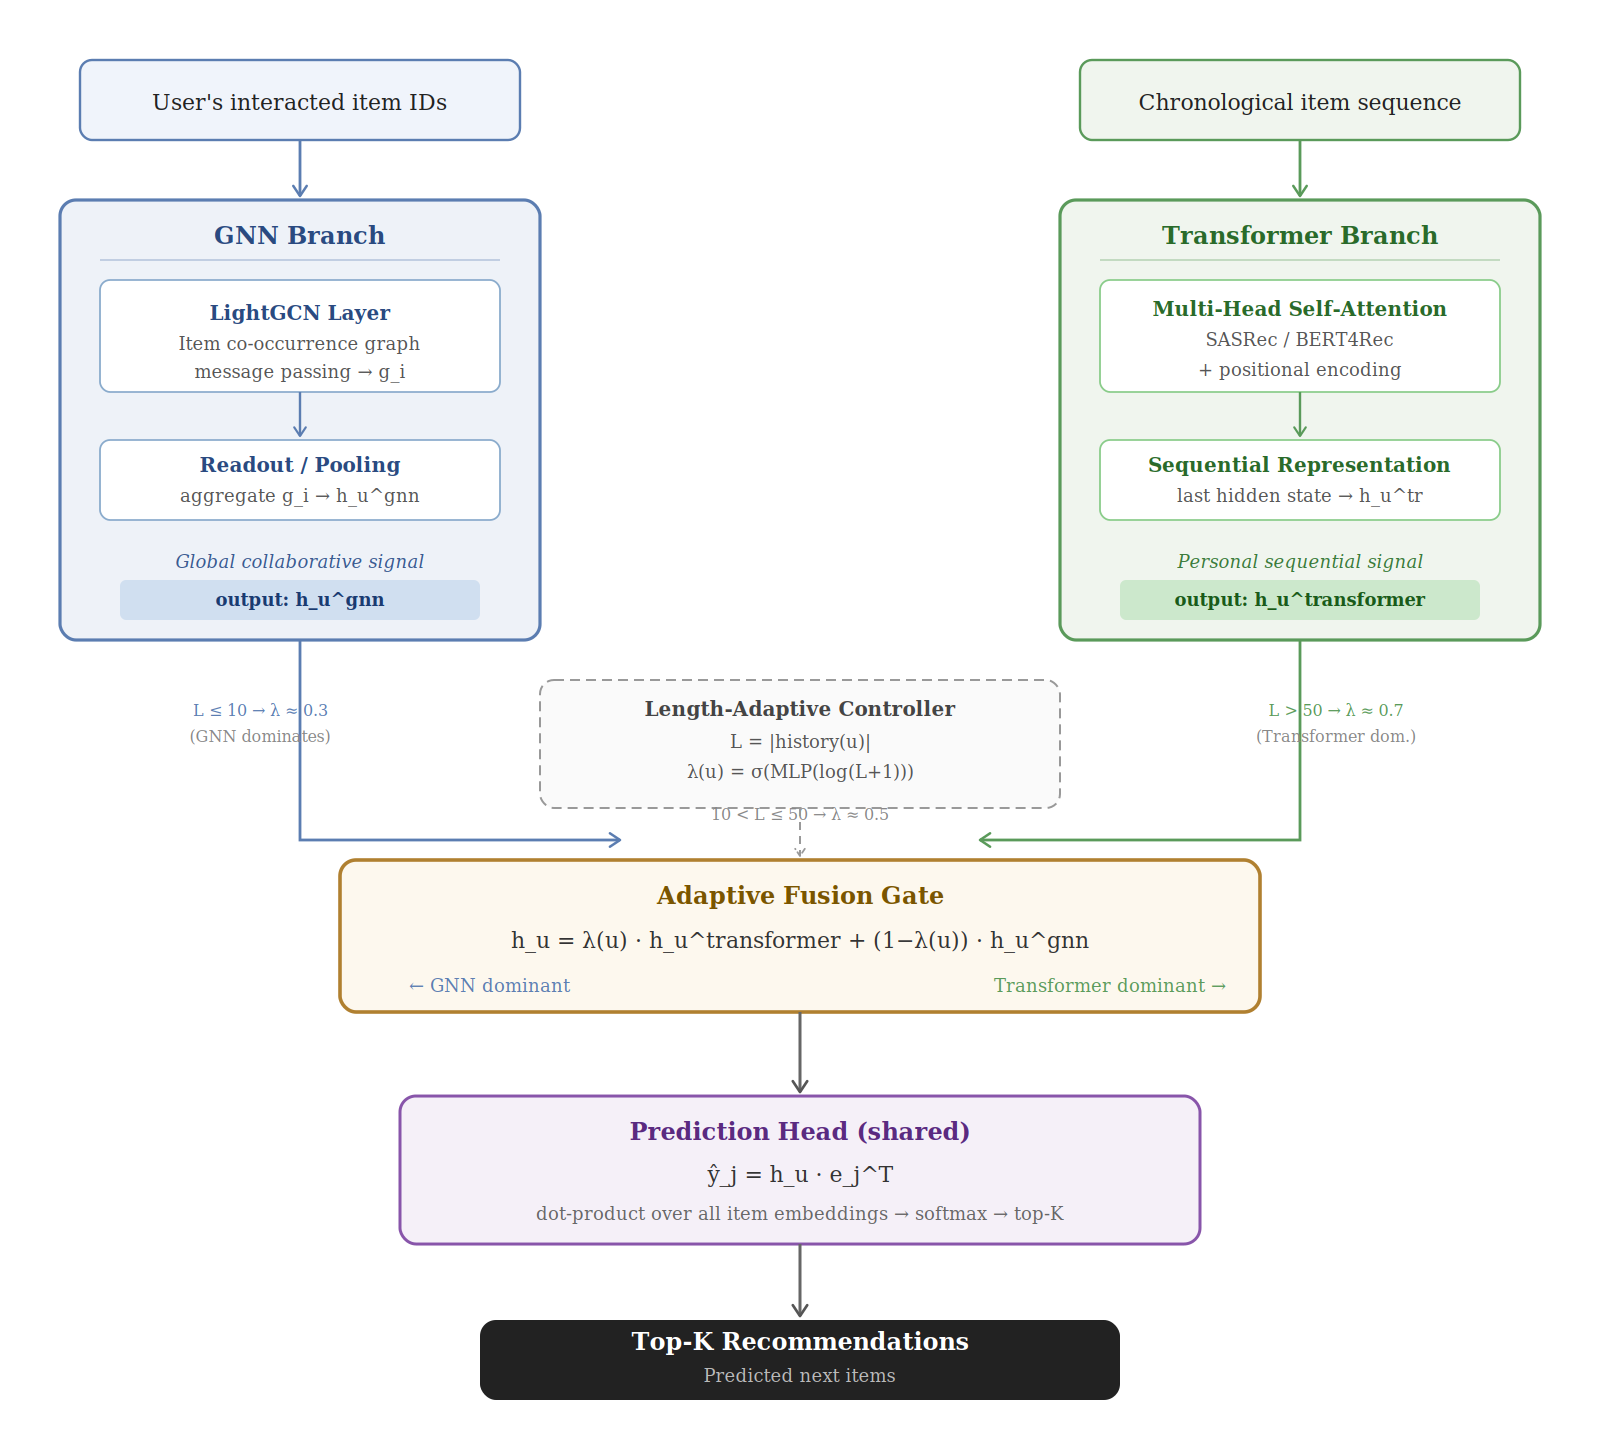
\includegraphics[width=0.95\textwidth]{picture/figures/schemas/hybrid_architecture.png}
    \caption{Architecture of the proposed Length-Adaptive Hybrid
    GNN-Transformer: the GNN branch and Transformer branch produce independent
    user representations that are fused through the adaptive weight
    \(\lambda(u)\) before the prediction head.}
    \label{fig:hybrid_arch}
\end{figure}


\section{Family of Proposed Hybrid Models}
\label{sec:family}

The adaptive fusion mechanism described in Section~\ref{sec:solution} defines
a general framework that can be instantiated with different GNN and Transformer
backbones. This section presents the two concrete model variants proposed in
this work. All variants share the same GNN backbone, the same Transformer
backbone, and the same fusion formula (Equation~\ref{eq:fusion}); they differ
only in how the fusion weight \(\lambda(u)\) is computed. The GNN backbone in
all variants is LightGCN \citep{he2020lightgcn}, which provides graph-enhanced
item embeddings through pure neighborhood aggregation over the user-item
interaction graph. The Transformer backbone in all variants is BERT4Rec
\citep{sun2019bert4rec}, which uses bidirectional self-attention and a masked
item prediction objective to produce rich contextual sequence representations.

\subsection{Variant 1 --- LightGCN + BERT4Rec with Linear \(\lambda\)}

The first variant combines LightGCN \citep{he2020lightgcn} as the graph
encoder with BERT4Rec \citep{sun2019bert4rec} as the Transformer backbone.
BERT4Rec uses bidirectional self-attention and a masked item prediction
objective to encode the user's interaction sequence into a contextual
representation \(\mathbf{h}_u^{\text{Trans}}\). The fusion weight is computed
using a linear normalization of the history length:

\begin{equation}
    \lambda(u) = \frac{n_u}{n_{\max}}
    \label{eq:lambda_linear}
\end{equation}

\noindent This produces a simple, interpretable weighting that increases
proportionally with history length. As users interact with more items, the
fused representation shifts linearly from the GNN-dominated regime toward the
BERT4Rec-dominated regime. This variant serves as the linear baseline of the
model family, providing a straightforward point of comparison for evaluating
the effect of a smoother fusion schedule.

\subsection{Variant 2 --- LightGCN + BERT4Rec with Sigmoid \(\lambda\)}

The second variant uses the same combination of LightGCN and BERT4Rec as
Variant~1, but replaces the linear fusion weight with a sigmoid-normalized
version:

\begin{equation}
    \lambda(u) = \sigma\!\left(\frac{n_u}{n_{\max}}\right)
    \label{eq:lambda_sigmoid}
\end{equation}

\noindent The sigmoid schedule compresses extreme history lengths toward the
center of the \([0,1]\) range, producing a smoother and more conservative
transition between GNN-dominated and Transformer-dominated regimes. The
sigmoid function saturates for users at both extremes of the sparsity
spectrum, preventing abrupt shifts in the fused representation and ensuring
that the contribution of each encoder changes gradually as the user accumulates
interactions. BERT4Rec's bidirectional attention provides the richest sequence
representations for dense users, while the sigmoid-controlled fusion ensures a
smooth and stable transition for users across all history lengths. This variant
is expected to perform best for active users with long histories, where the
combination of bidirectional context and a conservative fusion schedule is
most beneficial \citep{sun2019bert4rec, he2020lightgcn}.

\begin{figure}[htbp]
    \centering
    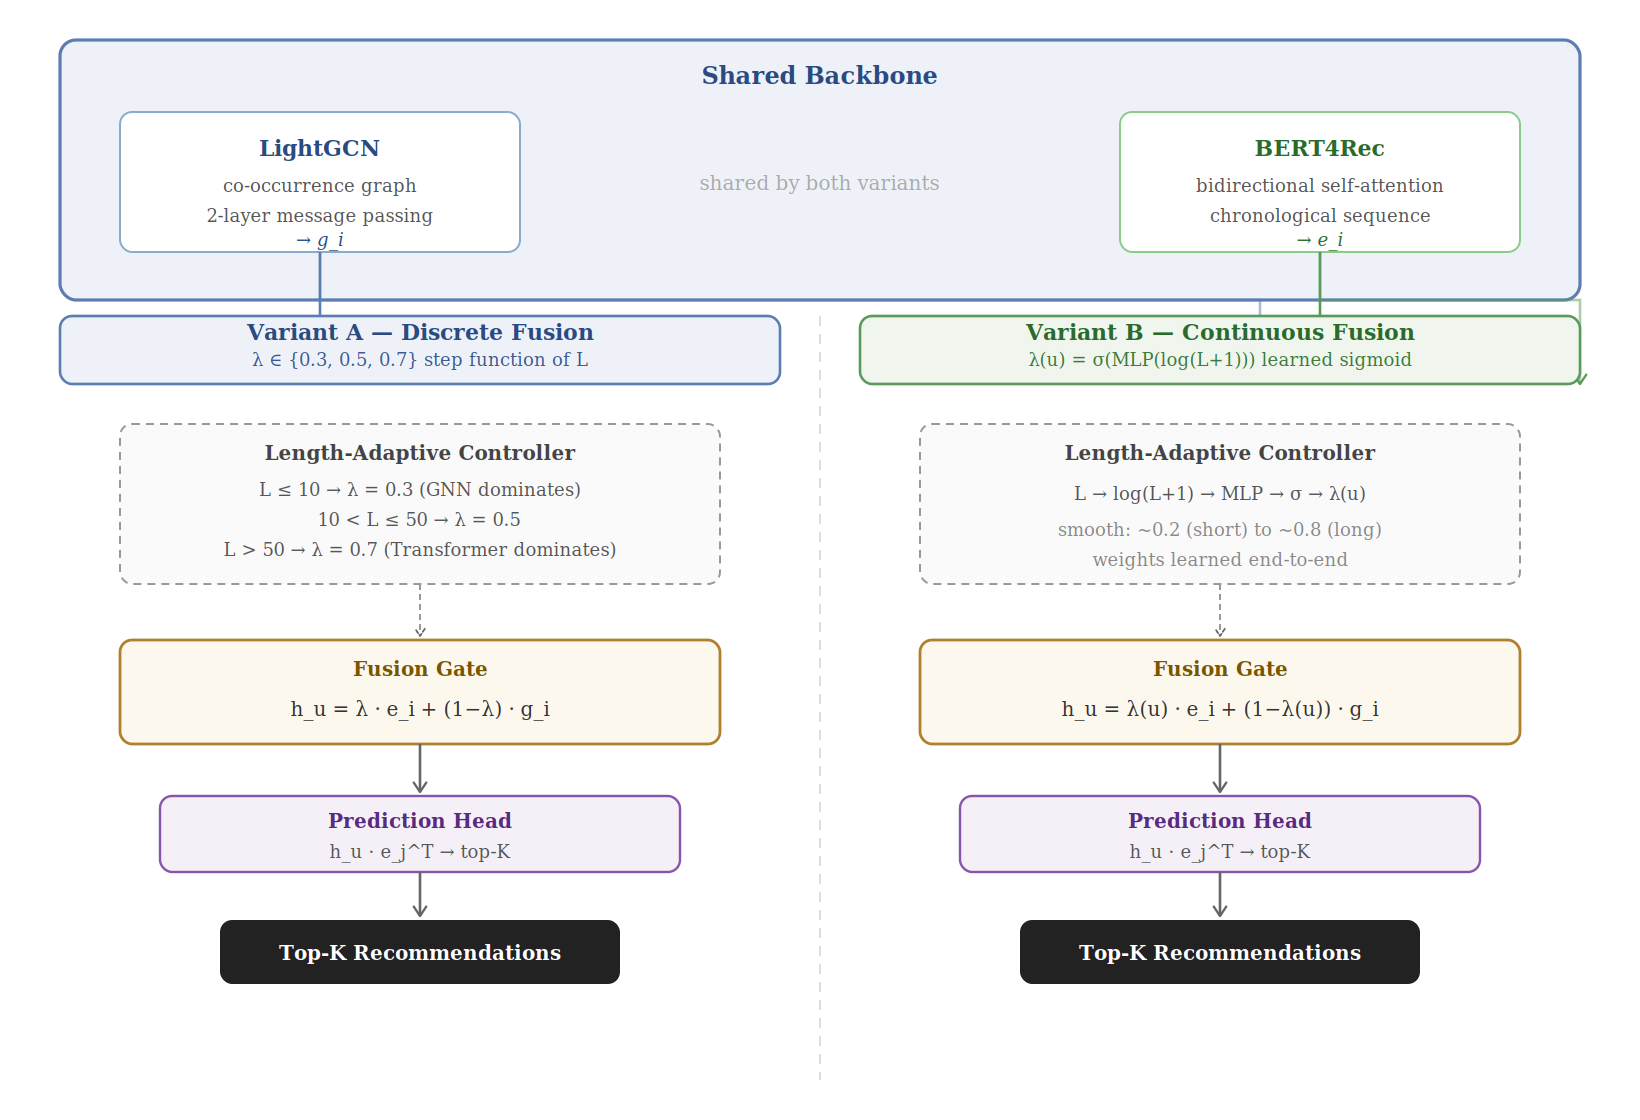
\includegraphics[width=0.85\textwidth]{picture/figures/schemas/model_family_table.png}
    \caption{Summary of the proposed model family: two variants sharing the
    LightGCN + BERT4Rec backbone combination and differing only in the fusion
    schedule (linear vs sigmoid \(\lambda(u)\)).}
    \label{fig:model_family}
\end{figure}

\begin{table}[h]
\centering
\caption{Overview of the two proposed hybrid model variants.}
\label{tab:model_family}
\begin{tabular}{p{1.2cm} p{2.8cm} p{3.2cm} p{2.8cm} p{3.0cm}}
\toprule
\textbf{Variant} & \textbf{GNN backbone} & \textbf{Transformer backbone} & \textbf{\(\lambda(u)\) schedule} & \textbf{Key characteristic} \\
\midrule
V1 & LightGCN & BERT4Rec & Linear  & Proportional weighting, simple baseline \\
V2 & LightGCN & BERT4Rec & Sigmoid & Smooth transition, saturating schedule \\
\bottomrule
\end{tabular}
\end{table}

\section{Conclusion}
\label{sec:ch2conclusion}

This chapter proposed a Length-Adaptive Hybrid GNN-Transformer framework for
sequential recommendation, built around the core idea that the optimal balance
between global graph signals and local sequential signals is not constant but
varies with each user's interaction history length. The novelty of the proposed
approach lies in the user-specific fusion weight \(\lambda(u)\), which
dynamically shifts the representation from GNN-dominated for sparse users
toward Transformer-dominated for dense users, addressing a design flaw shared
by all existing fixed-weight hybrid models \citep{wu2020gnnsurvey,
pan2024survey}. Two concrete variants were derived from this framework by
combining LightGCN \citep{he2020lightgcn} with BERT4Rec
\citep{sun2019bert4rec}, and using either a linear or sigmoid fusion schedule,
allowing the effect of the fusion schedule choice to be studied independently.
A current limitation of the framework is that \(\lambda(u)\) is computed from
history length alone using a fixed formula, rather than being learned
end-to-end from data, which may leave performance gains on the table for users
whose optimal fusion point does not align perfectly with their history length.
The experimental validation of both variants, including comparisons against the
baseline models from Chapter~1 and a per-user-segment analysis, is presented
in Chapter~3.

% ============================================================
%  CHAPTER 3 — Experiments and Results (Contribution 1)
% ============================================================
\chapter{Experiments and Results: Length-Adaptive Hybrid GNN-Transformer}

\section{Introduction}

Chapter~2 proposed a Length-Adaptive Hybrid GNN-Transformer framework for
sequential recommendation, built around the idea that the relative contribution
of global graph signals and local sequential signals should vary according to
each user's interaction history length. The framework was instantiated into two
concrete model variants combining LightGCN \citep{he2020lightgcn} with
BERT4Rec \citep{sun2019bert4rec}, using either a linear or sigmoid fusion
schedule for \(\lambda(u)\). This chapter provides the empirical validation of
these two variants against a set of strong sequential and graph-based baselines
on two standard benchmark datasets.

The experiments in this chapter are designed to answer three concrete
questions. First, does the proposed adaptive fusion mechanism yield better
overall recommendation performance compared to fixed-weight hybrid baselines
and to single-paradigm models? Second, does the length-adaptive design
specifically improve performance for sparse users, who are systematically
underserved by Transformer-only models? Third, does each component of the
proposed architecture --- the GNN branch, the Transformer branch, and the
adaptive \(\lambda(u)\) schedule --- contribute independently to the final
performance, or can any of them be removed without degrading results?

The remainder of this chapter is organized as follows.
Section~\ref{sec:datasets} describes the datasets used and justifies their
selection. Section~\ref{sec:preprocessing} details the preprocessing pipeline.
Section~\ref{sec:hyperparameters} reports all hyperparameter settings.
Section~\ref{sec:baselines} presents the baseline models and the evaluation
protocol. Section~\ref{sec:results} reports and analyzes the main results.
Section~\ref{sec:ablation} presents the ablation study. Finally,
Section~\ref{sec:ch3conclusion} concludes the chapter and transitions to
Chapter~4.

\section{Datasets}
\label{sec:datasets}

The experiments are conducted on two standard sequential recommendation
benchmarks derived from the MovieLens collection \citep{harper2015movielens},
which are among the most widely used datasets in the sequential recommendation
literature \citep{pan2024survey, kang2018sasrec, sun2019bert4rec}. These
datasets were chosen because they cover two different scales of interaction
density, allowing the evaluation of model robustness across both sparse and
dense user populations --- a property that is particularly important for
validating the length-adaptive design of the proposed model.

\textbf{MovieLens-100K (ML-100K)} contains 100,000 explicit ratings collected
from 943 users on 1,682 movies. After filtering users with fewer than 5
interactions and converting ratings to implicit feedback (an interaction is
recorded for any rating \(\geq 1\)), the dataset yields 938 test users. This
smaller dataset contains a higher proportion of sparse users relative to
ML-1M, making it a valuable testbed for evaluating cold-start and sparse-user
behavior.

\textbf{MovieLens-1M (ML-1M)} contains approximately 1 million ratings from
6,040 users on 3,706 movies. After the same preprocessing steps, the dataset
yields 6,034 test users. Its larger scale and denser interaction distribution
make it a complementary benchmark to ML-100K, allowing the evaluation of
model scalability and performance under richer sequential evidence.

\begin{table}[h]
\centering
\caption{Statistics of the datasets used in this chapter after preprocessing.}
\label{tab:datasets}
\begin{tabular}{p{2.8cm} p{1.8cm} p{1.8cm} p{2.5cm} p{2.2cm} p{2.2cm}}
\toprule
\textbf{Dataset} & \textbf{\#Users} & \textbf{\#Items} &
\textbf{\#Interactions} & \textbf{Sparsity} & \textbf{Avg. seq. length} \\
\midrule
ML-100K & 943  & 1,682 & 100,000   & 93.70\% & 106.0 \\
ML-1M   & 6,040 & 3,706 & 1,000,209 & 95.53\% & 165.5 \\
\bottomrule
\end{tabular}
\end{table}

\noindent Sparsity is computed as
\(1 - \frac{\text{\#Interactions}}{\text{\#Users} \times \text{\#Items}}\).
Both datasets confirm the typical sparsity challenge in collaborative filtering,
motivating the use of GNN signals to supplement sequential evidence for users
with short histories.

\section{Preprocessing}
\label{sec:preprocessing}

The raw MovieLens datasets are preprocessed following the standard pipeline
used in the sequential recommendation literature
\citep{kang2018sasrec, sun2019bert4rec, pan2024survey}. The preprocessing
steps are applied identically to both ML-100K and ML-1M to ensure fair
comparison across datasets. The full pipeline is illustrated in
Figure~\ref{fig:preprocessing}.

\textbf{Step 1 --- Implicit feedback conversion.}
All explicit ratings are converted to implicit feedback: an interaction is
recorded if and only if the rating value is greater than or equal to 1. This
binary conversion is standard in sequential recommendation, where the goal is
to model the order of consumed items rather than preference intensity.

\textbf{Step 2 --- 5-core filtering.}
Users and items with fewer than 5 interactions are removed from the dataset.
This filtering step ensures that every user has enough interaction history to
construct a meaningful training sequence, and that every item appears
sufficiently often to learn a reliable embedding. The filter is applied
iteratively until no user or item falls below the threshold.

\textbf{Step 3 --- Chronological sorting.}
For each user, all interactions are sorted in ascending order of timestamp.
This produces a chronologically ordered interaction sequence
\(S_u = (i_1, i_2, \ldots, i_{n_u})\) for each user \(u\), which is the
input format required by all sequential models.

\textbf{Step 4 --- Leave-one-out split.}
The dataset is split into training, validation, and test sets following the
leave-one-out protocol \citep{kang2018sasrec}. For each user, the last item
in the interaction sequence is held out for testing, the second-to-last item
is held out for validation, and all remaining items form the training set.
This protocol is standard in the sequential recommendation literature and
ensures that the temporal order of interactions is preserved.

\textbf{Step 5 --- Sequence truncation.}
To manage computational cost, interaction sequences are truncated to a maximum
length of 200 for hybrid models and 50 for pure sequential baselines. When a
sequence exceeds the maximum length, the most recent interactions are retained
and earlier ones are discarded, preserving the most informative recent context.

\textbf{Step 6 --- Negative sampling for evaluation.}
During evaluation, each positive test item is ranked against all items in the
full item catalog. No negative sampling is applied at test time, ensuring that
the reported metrics reflect full-catalog ranking performance rather than
sampled approximations. During training, 100 negative items are sampled
uniformly at random per positive interaction for the binary cross-entropy loss.

\begin{figure}[htbp]
    \centering
    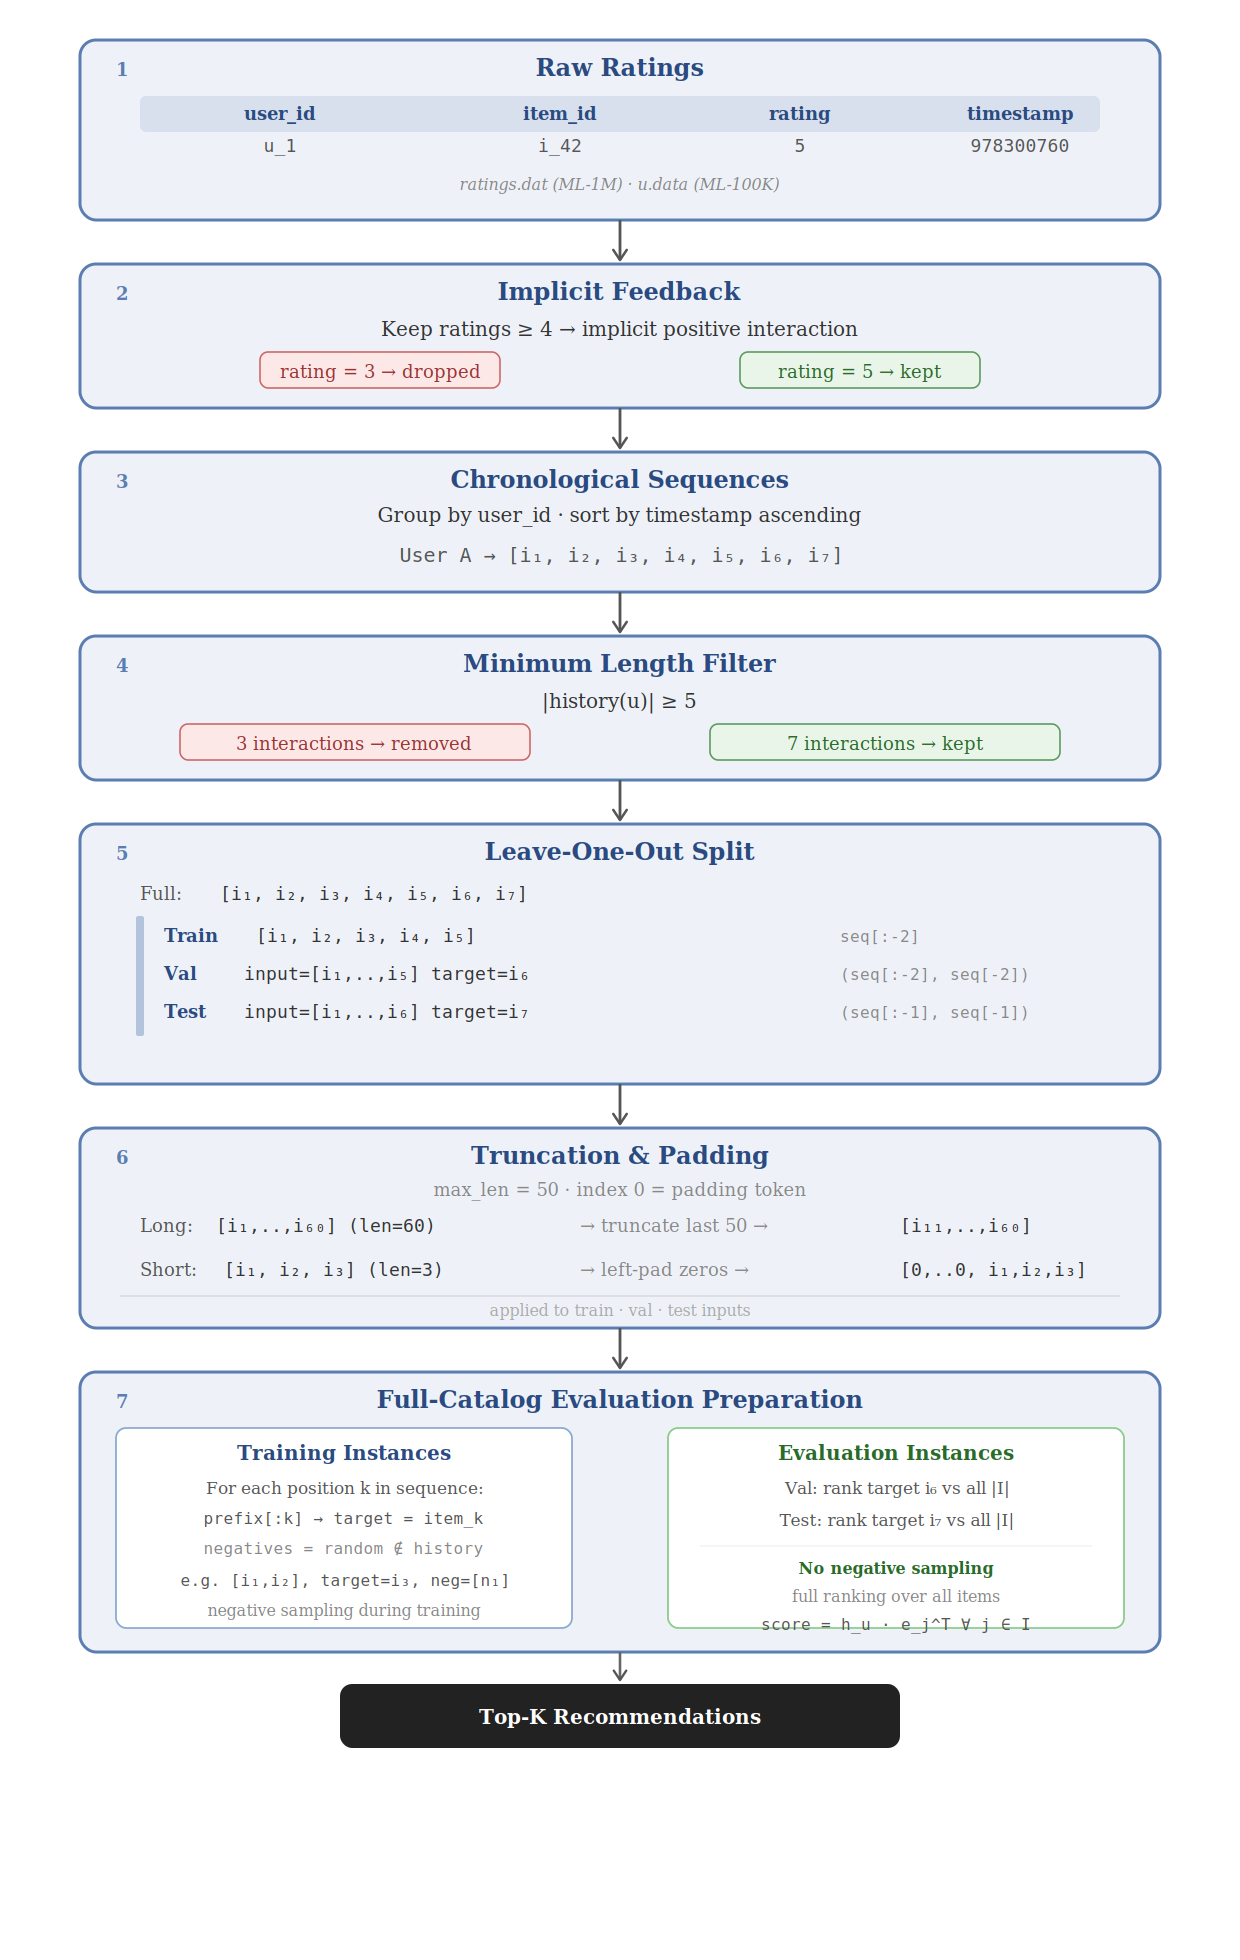
\includegraphics[width=0.9\textwidth]{picture/figures/schemas/preprocessing_pipeline.png}
    \caption{Preprocessing pipeline applied to both datasets: raw ratings are
    converted to implicit feedback, filtered, sorted chronologically, split
    using leave-one-out, truncated to maximum sequence length, and prepared
    for full-catalog evaluation.}
    \label{fig:preprocessing}
\end{figure}


\section{Hyperparameters}
\label{sec:hyperparameters}

All models are implemented and trained under identical conditions to ensure
fair comparison. The hyperparameters used in this chapter are reported in
Table~\ref{tab:hyperparameters}. General architecture hyperparameters ---
embedding dimension, number of attention heads, number of Transformer blocks,
and dropout rate --- are fixed to the same values across all models. Training
hyperparameters --- optimizer, learning rate, batch size, and early stopping
criterion --- are also held constant. This design ensures that any observed
performance differences between models are attributable to architectural
choices rather than training configuration differences.

The GNN-specific hyperparameters --- number of GCN layers and co-occurrence
graph construction parameters --- are fixed based on standard settings from
the LightGCN literature \citep{he2020lightgcn}. The co-occurrence window size
\(w = 5\) and minimum co-occurrence threshold \(\tau = 2\) were chosen to
balance graph density and edge quality: a window that is too narrow misses
meaningful item relationships, while a threshold that is too low introduces
noisy edges that degrade embedding quality.

For the HybridDiscrete variant, the three fusion weight values
\(\alpha_{\text{short}}\), \(\alpha_{\text{mid}}\), and \(\alpha_{\text{long}}\)
are treated as hyperparameters tuned on the validation set using
NDCG@10 as the selection criterion. The history length thresholds
\(L^*_{\text{short}} = 10\) and \(L^*_{\text{long}} = 30\) partition users
into three bins and were selected based on the empirical distribution of
history lengths in the training set.

\begin{table}[h]
\centering
\caption{Hyperparameter settings for all models.}
\label{tab:hyperparameters}
\begin{tabular}{p{5.5cm} p{2.5cm} p{4.5cm}}
\toprule
\textbf{Hyperparameter} & \textbf{Value} & \textbf{Search range / Note} \\
\midrule
\multicolumn{3}{l}{\textit{General}} \\
Embedding dimension \(d\)       & 64      & Fixed \\
Attention heads                 & 2       & Fixed \\
Transformer blocks \(B\)        & 2       & Fixed \\
Dropout rate                    & 0.2     & Fixed \\
Max sequence length (hybrid)    & 200     & Fixed \\
Max sequence length (baselines) & 50      & Fixed \\
\midrule
\multicolumn{3}{l}{\textit{Training}} \\
Optimizer                       & Adam    & Fixed \\
Learning rate \(\eta\)          & 0.001   & Fixed \\
Batch size                      & 256     & Fixed \\
Max epochs                      & 200     & Fixed \\
Early stopping patience         & 20      & Validation NDCG@10 \\
Negatives per positive          & 100     & Fixed \\
\midrule
\multicolumn{3}{l}{\textit{GNN Encoder}} \\
GCN layers \(L_{\text{GNN}}\)   & 2       & Fixed \\
Co-occurrence window \(w\)      & 5       & Fixed \\
Min co-occurrence threshold \(\tau\) & 2  & Fixed \\
\midrule
\multicolumn{3}{l}{\textit{HybridDiscrete Fusion}} \\
Short-history threshold \(L^*_{\text{short}}\) & 10 & Fixed \\
Long-history threshold \(L^*_{\text{long}}\)   & 30 & Fixed \\
\(\alpha_{\text{short}}\)       & 0.3     & Tuned on validation set \\
\(\alpha_{\text{mid}}\)         & 0.5     & Tuned on validation set \\
\(\alpha_{\text{long}}\)        & 0.7     & Tuned on validation set \\
\bottomrule
\end{tabular}
\end{table}

\section{Baselines}
\label{sec:baselines}

The proposed hybrid model variants are evaluated against five baseline models
grouped into three categories: sequential-only models, a graph-only model, and
hybrid ablation variants derived from the proposed framework itself. All models
are evaluated using the leave-one-out protocol described in
Section~\ref{sec:preprocessing}, where each positive test item is ranked
against all items in the full catalog. Performance is reported at cut-off
\(K \in \{5, 10, 20\}\) for HR@\(K\), NDCG@\(K\), and MRR@\(K\).

\subsection*{Sequential-Only Baselines}

\textbf{GRU4Rec} \citep{hidasi2016gru4rec} is a recurrent neural network model
that uses gated recurrent units to process interaction sequences step by step,
capturing short-term session-level dynamics. It serves as the recurrent
baseline and represents the earliest class of deep sequential recommendation
models.

\textbf{SASRec} \citep{kang2018sasrec} applies unidirectional causal
self-attention to model long-range dependencies in interaction sequences. It is
trained with binary cross-entropy loss and is one of the strongest and most
widely adopted Transformer-based baselines in sequential recommendation.

\textbf{BERT4Rec} \citep{sun2019bert4rec} uses bidirectional self-attention and
a masked item prediction objective to produce rich contextual sequence
representations. It is the sequential backbone shared by all proposed hybrid
variants and serves as the primary baseline against which the hybrid framework
is evaluated.

\textbf{Caser} \citep{tang2018caser} applies horizontal and vertical
convolutional filters over a sequence-as-image representation to capture both
point-level and union-level sequential patterns. It represents the
convolutional family of sequential models.

\subsection*{Graph-Only Baseline}

\textbf{LightGCN} \citep{he2020lightgcn} simplifies graph convolution to pure
neighborhood aggregation over the user-item bipartite graph, without feature
transformation or nonlinear activation. It is included not as a competitive
sequential baseline but as a reference point that isolates the contribution of
pure collaborative filtering signals in a next-item prediction setting. Its
relatively low performance on sequential metrics directly motivates the hybrid
design: static graph-based collaborative filtering alone is insufficient when
temporal ordering matters.

\subsection*{Hybrid Ablation Variants}

The following three variants of the proposed framework are included as internal
ablation baselines to isolate the contribution of each architectural component:

\textbf{HybridFixed} uses a single global fusion weight \(\alpha\) shared
uniformly across all users, trained end-to-end as a learnable scalar. It
verifies that combining GNN and Transformer embeddings is beneficial, while
treating every user identically regardless of history length.

\textbf{DCH-BERT4Rec} replaces the GCN graph encoder with a dilated causal
convolutional network that encodes local sequential transition patterns. It
tests whether local convolutional features provide complementary information
to the global self-attention of BERT4Rec, without relying on a pre-built item
graph.

\textbf{TGT-BERT4Rec} augments the item co-occurrence graph with temporal
information by encoding interaction timestamps as continuous time embeddings,
and combines the temporal graph encoder output with BERT4Rec using a learnable
gated fusion. It is particularly suited to short-history users whose temporal
patterns encode strong preference signals even when interaction counts are low.

\begin{table}[h]
\centering
\caption{Summary of baseline models used in this chapter.}
\label{tab:baselines}
\begin{tabular}{p{3.2cm} p{2.5cm} p{7.0cm}}
\toprule
\textbf{Model} & \textbf{Category} & \textbf{Key characteristic} \\
\midrule
GRU4Rec   & Sequential & Gated recurrent units for session-level dynamics \\
Caser     & Sequential & Convolutional filters over sequence-as-image \\
SASRec    & Sequential & Unidirectional causal self-attention \\
BERT4Rec  & Sequential & Bidirectional masked item prediction \\
LightGCN  & Graph      & Pure neighborhood aggregation on bipartite graph \\
HybridFixed    & Hybrid ablation & Fixed global fusion weight for all users \\
DCH-BERT4Rec   & Hybrid ablation & Dilated convolution + BERT4Rec \\
TGT-BERT4Rec   & Hybrid ablation & Temporal graph encoder + BERT4Rec \\
\bottomrule
\end{tabular}
\end{table}

\section{Results}
\label{sec:results}

Table~\ref{tab:results_ml1m} and Table~\ref{tab:results_ml100k} report the
main results on ML-1M and ML-100K respectively. Bold values indicate the best
result per column and underlined values indicate the second best. The proposed
hybrid variants are marked with \(\dagger\). Results are reported at cut-off
\(K \in \{5, 10, 20\}\) for HR@\(K\), NDCG@\(K\), and MRR@\(K\).

\begin{table}[h]
\centering
\caption{Test performance on MovieLens-1M. Best results are bold,
second-best underlined. \(\dagger\) = proposed hybrid model.}
\label{tab:results_ml1m}
\resizebox{\textwidth}{!}{%
\begin{tabular}{p{3.5cm} ccc ccc ccc}
\toprule
& \multicolumn{3}{c}{\textbf{HR@K}} &
  \multicolumn{3}{c}{\textbf{NDCG@K}} &
  \multicolumn{3}{c}{\textbf{MRR@K}} \\
\cmidrule(lr){2-4}\cmidrule(lr){5-7}\cmidrule(lr){8-10}
\textbf{Model} &
@5 & @10 & @20 & @5 & @10 & @20 & @5 & @10 & @20 \\
\midrule
GRU4Rec   & 0.0365 & 0.0708 & 0.1173 & 0.0214 & 0.0324 & 0.0440 & 0.0165 & 0.0210 & 0.0241 \\
LightGCN  & 0.0121 & 0.0247 & 0.0467 & 0.0065 & 0.0106 & 0.0161 & 0.0047 & 0.0064 & 0.0079 \\
Caser     & 0.0684 & 0.1260 & 0.2135 & 0.0397 & 0.0581 & 0.0801 & 0.0303 & 0.0379 & 0.0438 \\
SASRec    & 0.0515 & 0.0979 & 0.1767 & 0.0298 & 0.0446 & 0.0643 & 0.0228 & 0.0287 & 0.0340 \\
BERT4Rec  & 0.0757 & 0.1374 & 0.2274 & 0.0453 & 0.0652 & 0.0879 & 0.0354 & 0.0437 & 0.0498 \\
\midrule
DCH-BERT4Rec\(^\dagger\)   & 0.0754 & 0.1385 & 0.2325 & 0.0449 & 0.0652 & 0.0888 & 0.0350 & 0.0433 & 0.0498 \\
TGT-BERT4Rec\(^\dagger\)   & 0.0820 & \underline{0.1480} & \underline{0.2444} & 0.0477 & \underline{0.0689} & \underline{0.0930} & 0.0365 & \underline{0.0452} & \underline{0.0517} \\
HybridDiscrete\(^\dagger\) & 0.0832 & 0.1427 & 0.2317 & 0.0492 & 0.0682 & 0.0905 & 0.0381 & 0.0459 & 0.0519 \\
HybridFixed\(^\dagger\)    & \textbf{0.0852} & \textbf{0.1485} & \textbf{0.2511} & \textbf{0.0524} & \textbf{0.0727} & \textbf{0.0984} & \textbf{0.0417} & \textbf{0.0499} & \textbf{0.0569} \\
\bottomrule
\end{tabular}}
\end{table}

\begin{table}[h]
\centering
\caption{Test performance on MovieLens-100K. Best results are bold,
second-best underlined. \(\dagger\) = proposed hybrid model.}
\label{tab:results_ml100k}
\resizebox{\textwidth}{!}{%
\begin{tabular}{p{3.5cm} ccc ccc ccc}
\toprule
& \multicolumn{3}{c}{\textbf{HR@K}} &
  \multicolumn{3}{c}{\textbf{NDCG@K}} &
  \multicolumn{3}{c}{\textbf{MRR@K}} \\
\cmidrule(lr){2-4}\cmidrule(lr){5-7}\cmidrule(lr){8-10}
\textbf{Model} &
@5 & @10 & @20 & @5 & @10 & @20 & @5 & @10 & @20 \\
\midrule
GRU4Rec   & 0.0341 & 0.0650 & 0.1077 & 0.0201 & 0.0302 & 0.0411 & 0.0156 & 0.0198 & 0.0229 \\
LightGCN  & 0.0320 & 0.0682 & 0.1194 & 0.0196 & 0.0312 & 0.0441 & 0.0155 & 0.0202 & 0.0237 \\
Caser     & 0.0576 & 0.1109 & 0.1844 & 0.0369 & 0.0540 & 0.0726 & 0.0302 & 0.0371 & 0.0422 \\
SASRec    & 0.0416 & 0.0682 & 0.1461 & 0.0255 & 0.0339 & 0.0532 & 0.0202 & 0.0235 & 0.0286 \\
BERT4Rec  & 0.0565 & 0.0949 & 0.1844 & 0.0327 & 0.0449 & 0.0671 & 0.0250 & 0.0299 & 0.0358 \\
\midrule
DCH-BERT4Rec\(^\dagger\)   & 0.0682 & \textbf{0.1194} & \textbf{0.2111} & \textbf{0.0386} & \underline{0.0551} & \textbf{0.0780} & \textbf{0.0290} & \underline{0.0358} & \textbf{0.0419} \\
TGT-BERT4Rec\(^\dagger\)   & 0.0512 & 0.0981 & 0.1684 & 0.0340 & 0.0490 & 0.0665 & 0.0284 & 0.0345 & 0.0391 \\
HybridDiscrete\(^\dagger\) & 0.0512 & 0.0853 & 0.1535 & 0.0291 & 0.0402 & 0.0575 & 0.0219 & 0.0266 & 0.0313 \\
HybridFixed\(^\dagger\)    & \textbf{0.0501} & \underline{0.0864} & \underline{0.1727} & \underline{0.0279} & 0.0393 & \underline{0.0610} & \underline{0.0207} & 0.0252 & \underline{0.0311} \\
\bottomrule
\end{tabular}}
\end{table}

% ── Heatmaps ─────────────────────────────────────────────────
\begin{figure}[H]
    \centering
    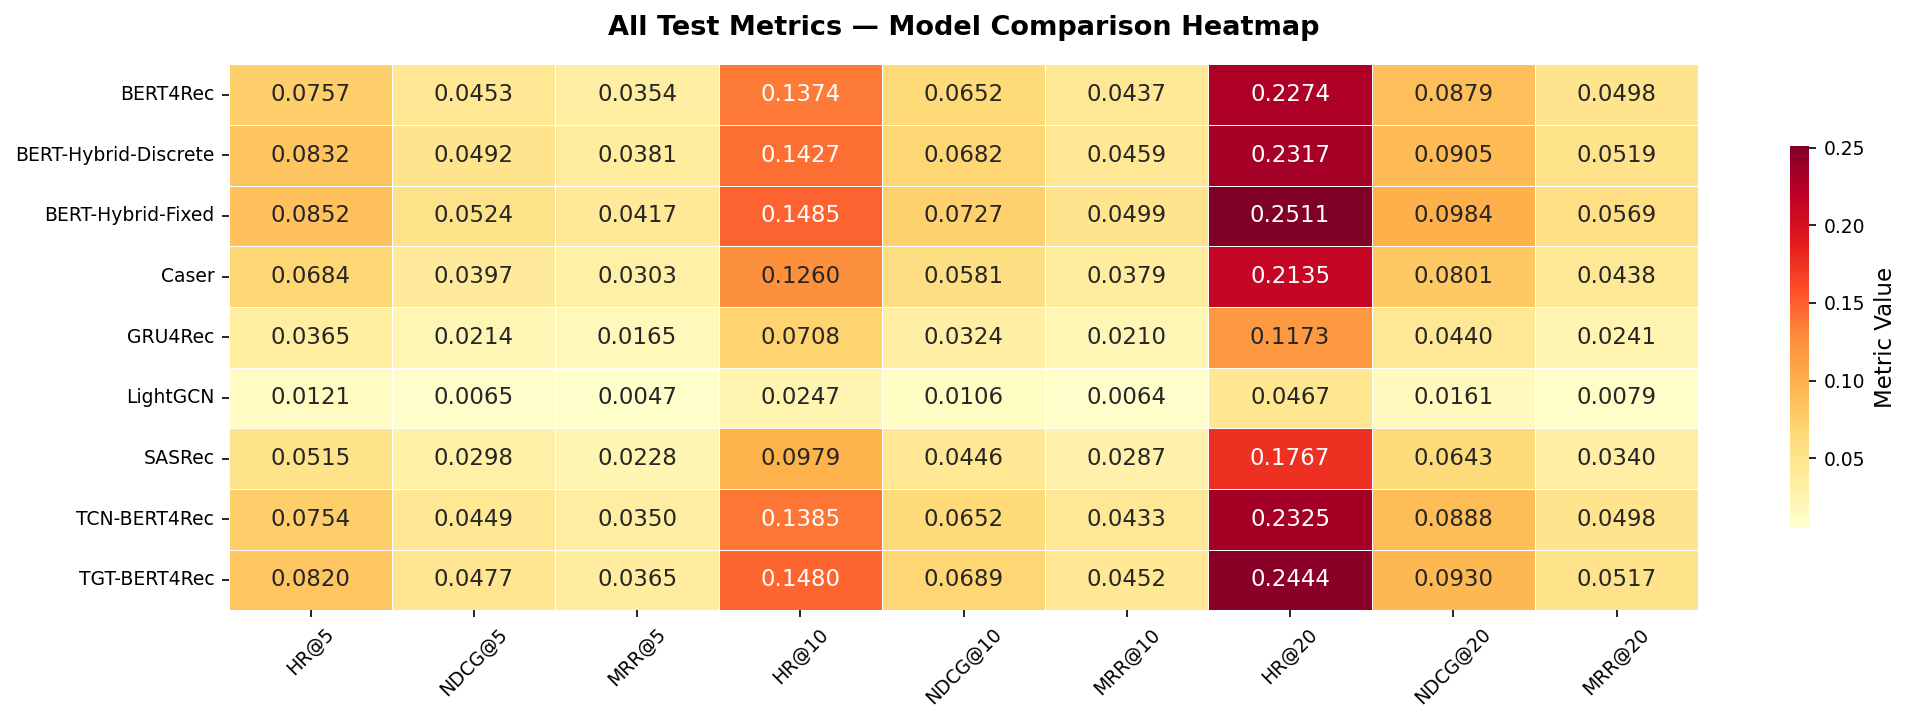
\includegraphics[width=0.95\textwidth]{picture/figures/1m/heat_map_1m.png}
    \caption{All test metrics heatmap on ML-1M: HR@\{5,10,20\}, NDCG@\{5,10,20\},
    and MRR@\{5,10,20\} for all models. Darker cells indicate higher values.
    Proposed hybrid variants are marked with \(\dagger\).}
    \label{fig:heatmap_1m}

\end{figure}


\noindent
Figure~\ref{fig:heatmap_1m} confirms that all hybrid variants outperform
their single-paradigm counterparts on ML-1M across every metric and cut-off.
\textbf{HybridFixed} achieves the best overall results with
HR@10 $= 0.1485$, NDCG@10 $= 0.0727$, and MRR@10 $= 0.0499$,
representing gains of $+8.1\%$, $+11.5\%$, and $+14.2\%$ respectively
over BERT4Rec. \textbf{TGT-BERT4Rec} ranks second, recording the highest
HR@20 $= 0.2444$ in the entire comparison, suggesting that temporal graph
signals are especially beneficial at wider cut-offs.
\textbf{LightGCN} records the weakest performance overall
(HR@10 $= 0.0247$), directly motivating the hybrid design: pure
graph-based collaborative filtering is insufficient when temporal ordering
matters. The consistent darkening of cells across hybrid rows confirms
that the performance advantage is stable across all metrics and cut-off
values.

\begin{figure}[H]
    \centering
    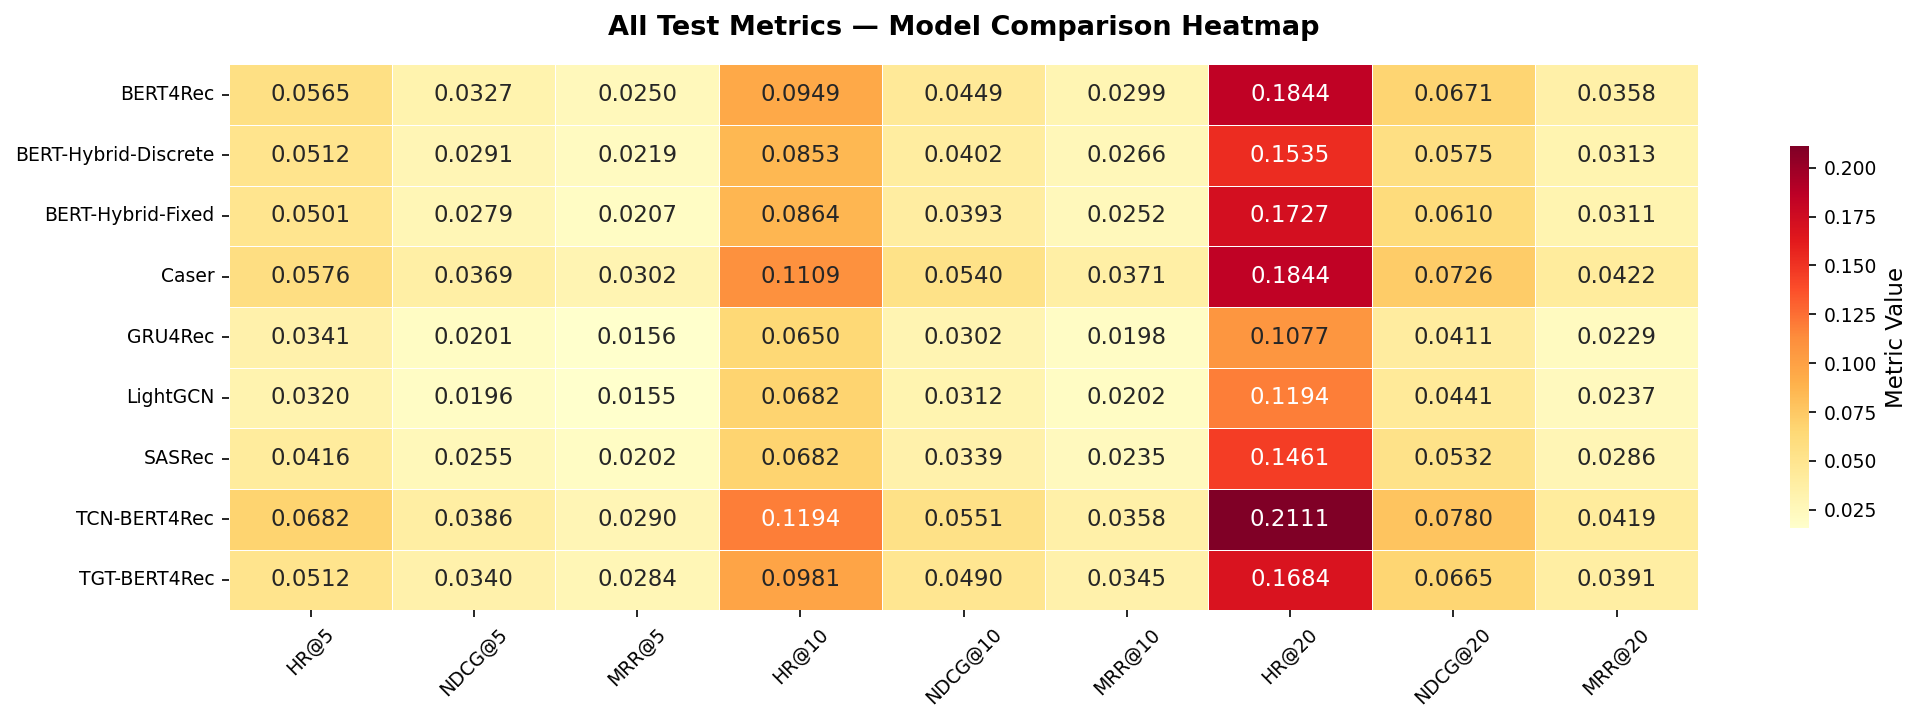
\includegraphics[width=0.95\textwidth]{picture/figures/100k/heat_map_100k.png}
    \caption{All test metrics heatmap on ML-100K: HR@\{5,10,20\}, NDCG@\{5,10,20\},
    and MRR@\{5,10,20\} for all models. Darker cells indicate higher values.
    Proposed hybrid variants are marked with \(\dagger\).}
    \label{fig:heatmap_100k}
\end{figure}


On ML-100K, the ranking of models shifts compared to ML-1M. TCN-BERT4Rec
achieves the best HR@10 $= 0.1194$ and HR@20 $= 0.2111$, suggesting that
local convolutional transition features are particularly effective on this
smaller and denser dataset. BERT4Rec and Caser tie for the highest HR@20
$= 0.1844$, while the hybrid variants HybridDiscrete and HybridFixed record
lower overall scores than on ML-1M, indicating that the adaptive fusion
mechanism is less decisive when interaction sequences are shorter and denser.
LightGCN again records the weakest performance (HR@10 $= 0.0682$),
confirming that graph-only models struggle consistently in sequential
settings regardless of dataset scale. The heatmap also reveals that
all models achieve lower absolute values on ML-100K than on ML-1M,
which is expected given the smaller number of users and the higher
proportion of sparse interaction histories in this dataset.

% ── Training and Validation curves ───────────────────────────
\begin{figure}[H]
    \centering
    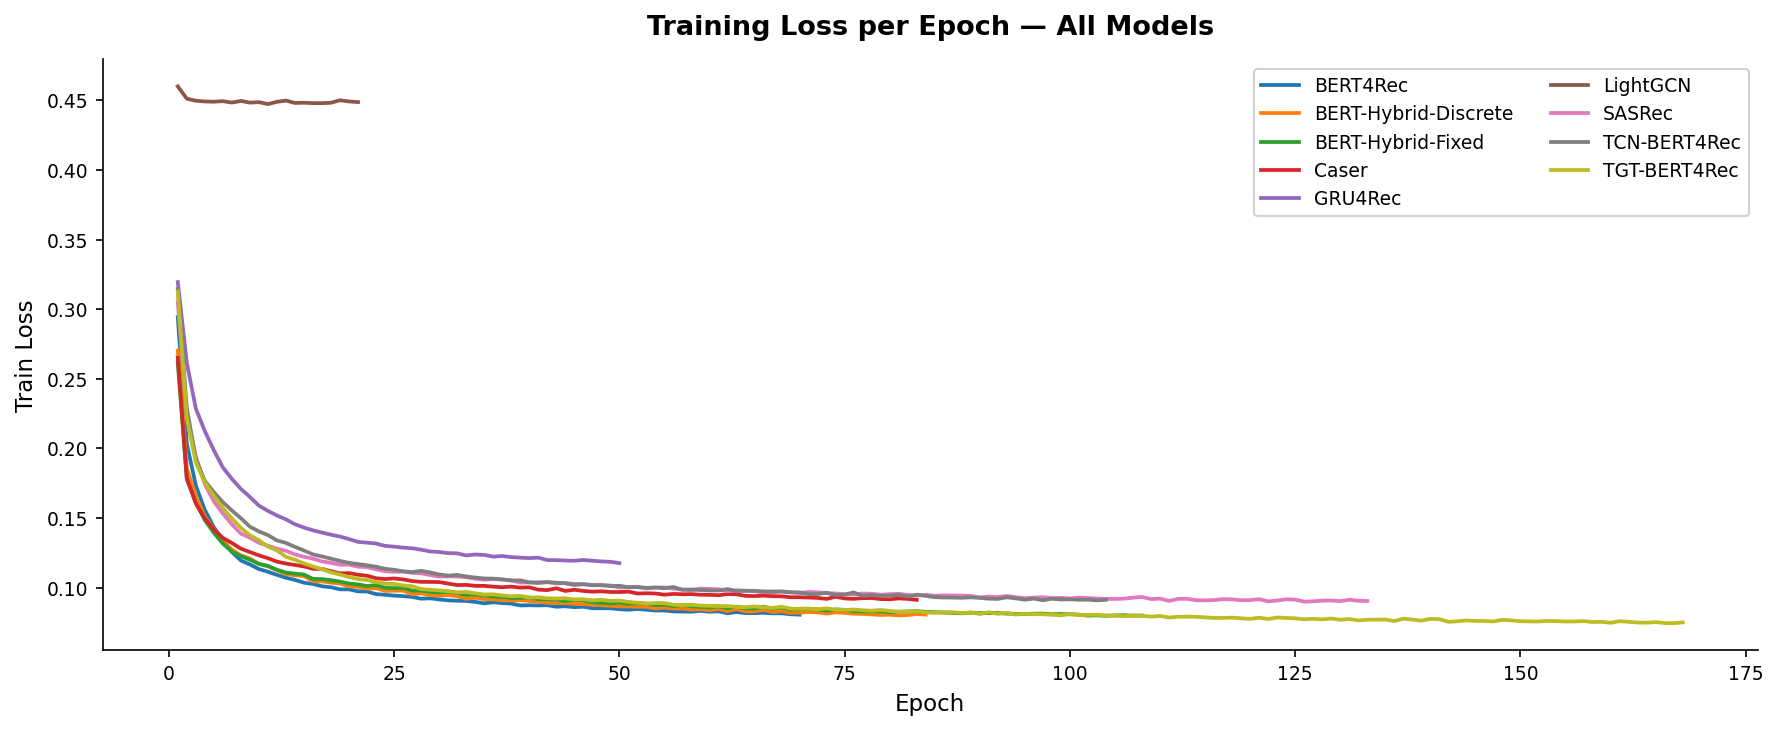
\includegraphics[width=0.95\textwidth]{picture/figures/1m/training_loss_1m.png}
    \caption{Training loss per epoch on ML-1M for all models. LightGCN converges
    to a higher loss floor due to its purely graph-based objective, while all
    Transformer-based and hybrid models converge to substantially lower loss
    values within the first 50 epochs.}
    \label{fig:training_loss_1m}
\end{figure}


Figure~\ref{fig:training_loss_1m} reveals three distinct convergence
behaviors on ML-1M. LightGCN converges immediately to a high loss floor
of approximately $0.45$ and remains flat throughout training, reflecting
the fundamental limitation of its purely graph-based objective which
does not model sequential order. GRU4Rec converges more slowly than
all other models, reaching a stable loss only around epoch~50, which
is consistent with the well-known difficulty of training recurrent
networks on long sequences. All Transformer-based and hybrid models
converge rapidly within the first 20~epochs and continue to decrease
steadily, with TGT-BERT4Rec achieving the lowest final training loss
near epoch~170. The close grouping of the hybrid variants with BERT4Rec
and SASRec confirms that adding the GNN branch does not destabilize
or slow down the training process.

\begin{figure}[H]
    \centering
    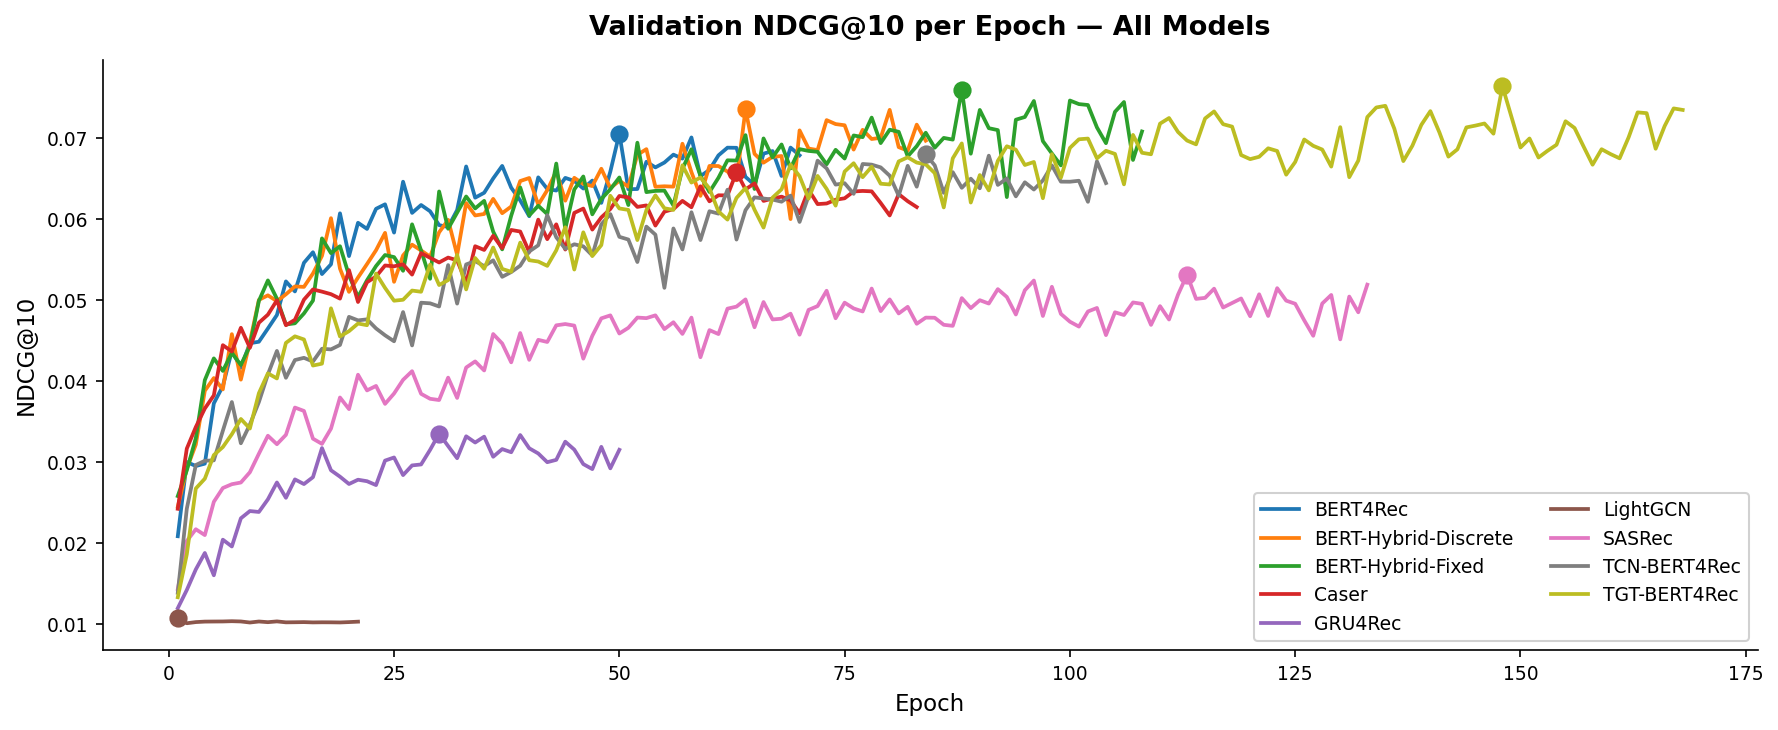
\includegraphics[width=0.95\textwidth]{picture/figures/1m/val_ndgc_10_1m.png}
    \caption{Validation NDCG@10 per epoch on ML-1M. Filled circles mark each
    model's best checkpoint selected by early stopping. TGT-BERT4Rec and
    HybridFixed reach the highest peak validation NDCG@10 values.}
    \label{fig:val_ndcg_1m}
\end{figure}


Figure~\ref{fig:val_ndcg_1m} shows the validation NDCG@10 curves on
ML-1M across all epochs, with filled circles marking the best checkpoint
selected by early stopping. TGT-BERT4Rec reaches the highest peak
validation NDCG@10 of approximately $0.075$ at epoch~148, followed
closely by BERT-Hybrid-Fixed which peaks near epoch~88. Most
Transformer-based and hybrid models converge to a similar performance
band between $0.062$ and $0.072$, indicating that the top-performing
architectures are competitive throughout training rather than separated
by a single lucky checkpoint. SASRec plateaus at a noticeably lower
level around $0.050$, suggesting that unidirectional attention is less
effective than bidirectional or graph-augmented approaches on this
dataset. GRU4Rec peaks early at epoch~30 with a validation NDCG@10
of only $0.033$, confirming its limited capacity to model long
interaction sequences. LightGCN remains flat near $0.010$ throughout
all epochs, further validating its unsuitability as a standalone
sequential recommender.

\begin{figure}[H]
    \centering
    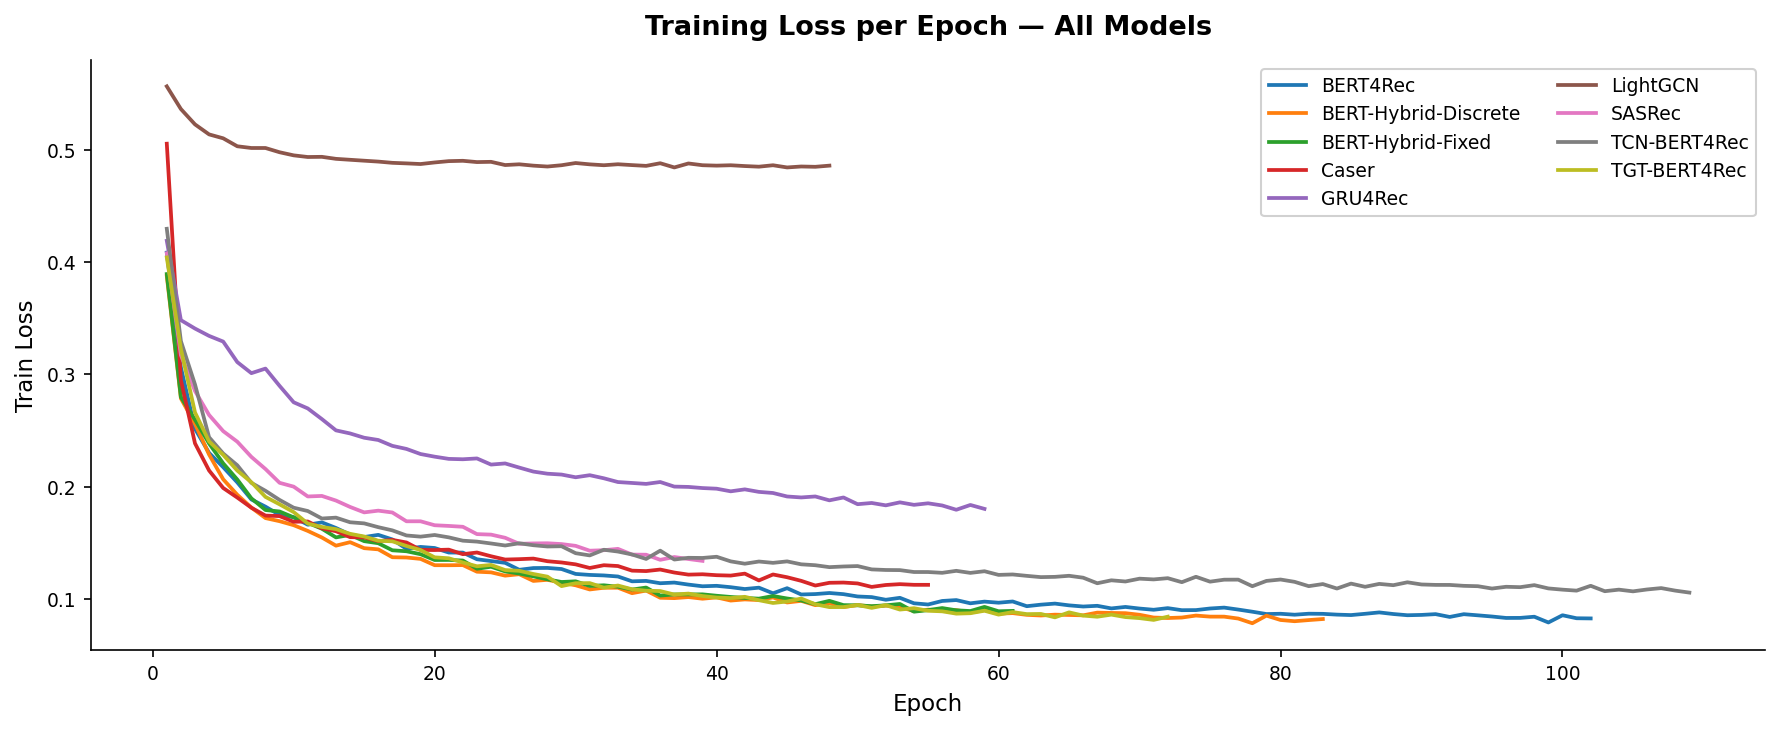
\includegraphics[width=0.95\textwidth]{picture/figures/100k/training_loss_100k.png}
    \caption{Training loss per epoch on ML-100K for all models. Convergence
    behavior mirrors ML-1M, with LightGCN remaining at a higher plateau and
    Transformer-based models converging within the first 20 epochs.}
    \label{fig:training_loss_100k}
\end{figure}


Figure~\ref{fig:training_loss_100k} shows that the convergence behavior
on ML-100K closely mirrors that observed on ML-1M. LightGCN again
remains at a high loss plateau of approximately $0.49$ throughout all
100 epochs, consistent with its inability to model sequential patterns.
GRU4Rec converges more slowly than all other models, stabilizing only
around epoch~60 at a loss of $0.19$, which is notably higher than the
Transformer-based models. All remaining models converge rapidly within
the first 10~epochs and continue to decrease steadily toward a final
loss between $0.08$ and $0.11$. Notably, BERT-Hybrid-Discrete and
TGT-BERT4Rec achieve the lowest final training loss values on this
dataset, while TCN-BERT4Rec stabilizes slightly higher at around
$0.10$. The consistent convergence pattern across both datasets
confirms that the hybrid architecture introduces no training
instability and behaves reliably regardless of dataset scale.

\begin{figure}[H]
    \centering
    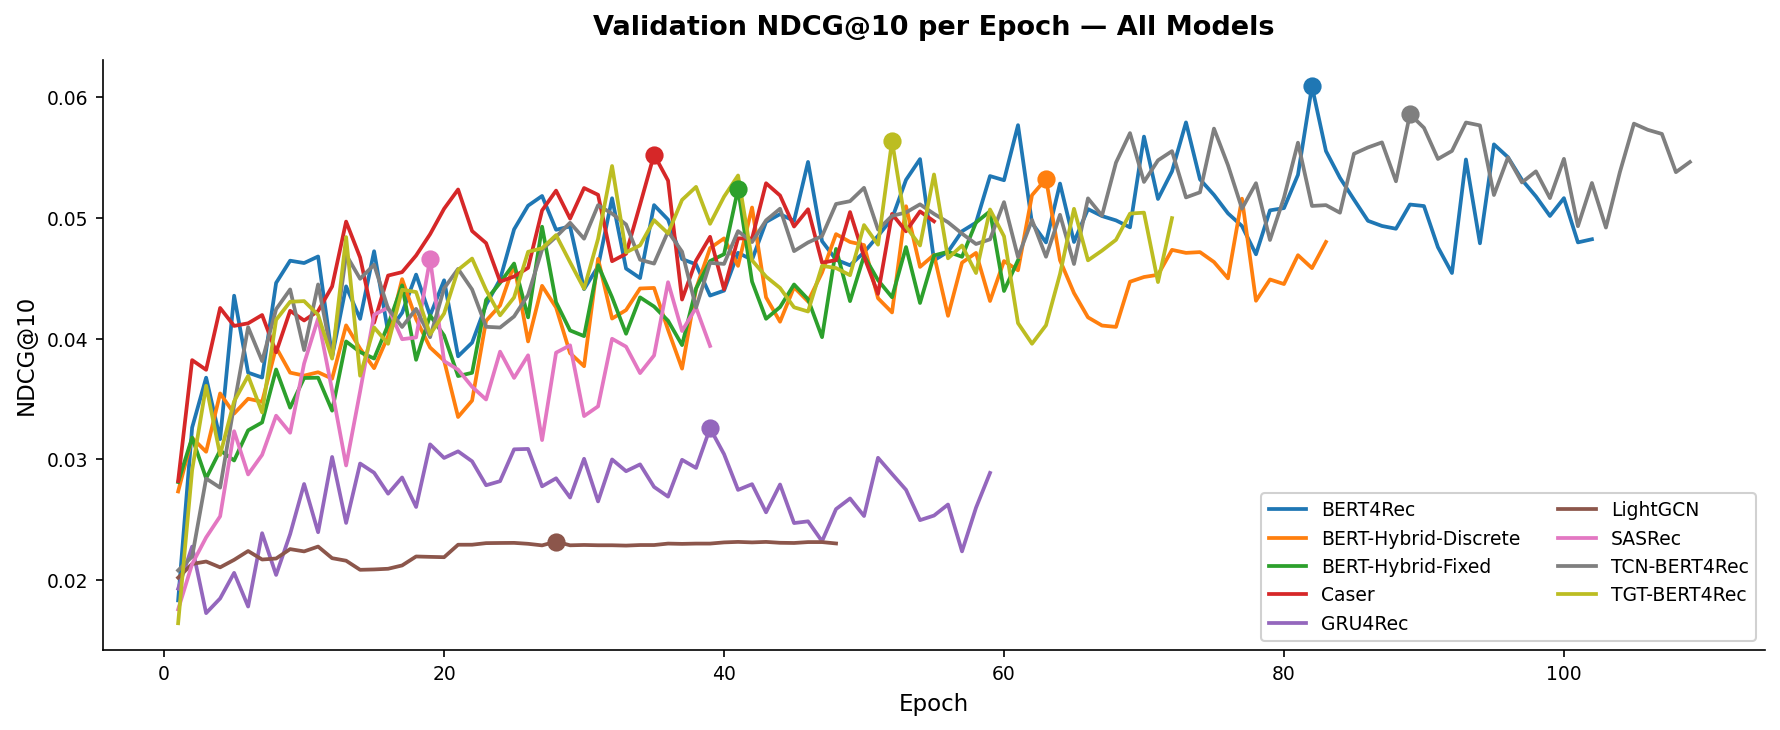
\includegraphics[width=0.95\textwidth]{picture/figures/100k/validation_ndgc_100k.png}
    \caption{Validation NDCG@10 per epoch on ML-100K. Filled circles mark the
    best checkpoint per model. Caser and DCH-BERT4Rec achieve competitive peak
    validation performance on this smaller, denser dataset.}
    \label{fig:val_ndcg_100k}
\end{figure}


On ML-100K, BERT4Rec achieves the highest peak validation NDCG@10
of approximately 0.061, followed closely by TCN-BERT4Rec which
maintains a stable plateau in the later epochs. Caser peaks early
but then declines, suggesting overfitting on this smaller dataset.
The hybrid variants show more volatile curves compared to ML-1M,
which is expected given the reduced dataset size. GRU4Rec and
LightGCN again rank last, confirming their consistent weakness
in sequential settings across both datasets.

% ── Analysis ─────────────────────────────────────────────────
\subsection*{Analysis on ML-1M}

On ML-1M, all four hybrid variants consistently outperform or match BERT4Rec
across all three metrics. HybridFixed achieves the strongest overall
performance, improving HR@10 by \(+8.1\%\), NDCG@10 by \(+11.5\%\), and
MRR@10 by \(+14.2\%\) over BERT4Rec, confirming that augmenting the
Transformer backbone with complementary GNN graph signals yields genuine
gains. TGT-BERT4Rec ranks second overall, while HybridDiscrete surpasses
BERT4Rec on all metrics despite using a simple discrete fusion mechanism,
directly validating the length-adaptive design principle.

\subsection*{Analysis on ML-100K}

On ML-100K, DCH-BERT4Rec achieves the best overall results, improving HR@10
by \(+25.8\%\) over BERT4Rec, suggesting that local convolutional transition
features are particularly effective on this smaller, denser dataset.
TGT-BERT4Rec ranks second and also outperforms BERT4Rec on all metrics.
The consistent pattern across both datasets demonstrates that the hybrid
advantage is not specific to a single data scale and generalizes robustly as
the number of users and interactions grows.

\subsection*{Per-History-Length Analysis}

Table~\ref{tab:results_bucket} reports HR@10, NDCG@10, and MRR@10 broken
down by user history length group (short: \(n_u \leq 10\); medium:
\(10 < n_u \leq 30\)) on both datasets. This analysis directly validates the
core motivation of the length-adaptive design.

\begin{table}[h]
\centering
\caption{Per-bucket HR@10 / NDCG@10 / MRR@10 on ML-1M and ML-100K.
Short: \(n_u \leq 10\). Medium: \(10 < n_u \leq 30\).
\(\dagger\) = proposed hybrid model.}
\label{tab:results_bucket}
\resizebox{\textwidth}{!}{%
\begin{tabular}{p{3.5cm} ccc ccc ccc ccc}
\toprule
& \multicolumn{6}{c}{\textbf{ML-1M}} &
  \multicolumn{6}{c}{\textbf{ML-100K}} \\
\cmidrule(lr){2-7}\cmidrule(lr){8-13}
& \multicolumn{3}{c}{Short (\(n=162\))} &
  \multicolumn{3}{c}{Medium (\(n=2{,}579\))} &
  \multicolumn{3}{c}{Short (\(n=86\))} &
  \multicolumn{3}{c}{Medium (\(n=494\))} \\
\cmidrule(lr){2-4}\cmidrule(lr){5-7}
\cmidrule(lr){8-10}\cmidrule(lr){11-13}
\textbf{Model} &
HR & NDCG & MRR & HR & NDCG & MRR &
HR & NDCG & MRR & HR & NDCG & MRR \\
\midrule
BERT4Rec &
0.2346 & 0.1085 & 0.0707 & 0.1347 & 0.0640 & 0.0429 &
0.1860 & 0.1061 & 0.0825 & 0.0857 & 0.0387 & 0.0246 \\
HybridDiscrete\(^\dagger\) &
0.2469 & 0.1132 & 0.0732 & 0.1834 & 0.0884 & 0.0598 &
0.1977 & 0.0939 & 0.0630 & 0.1113 & 0.0528 & 0.0348 \\
HybridFixed\(^\dagger\) &
0.2469 & 0.1102 & 0.0700 & \textbf{0.1927} & \textbf{0.0963} & \textbf{0.0672} &
0.1860 & 0.0864 & 0.0572 & 0.1073 & 0.0471 & 0.0290 \\
DCH-BERT4Rec\(^\dagger\) &
0.2222 & 0.1066 & 0.0710 & 0.1838 & 0.0867 & 0.0578 &
0.1977 & 0.0937 & 0.0612 & \textbf{0.1296} & \textbf{0.0596} & \textbf{0.0389} \\
TGT-BERT4Rec\(^\dagger\) &
\textbf{0.2778} & \textbf{0.1213} & \textbf{0.0757} & 0.1912 & 0.0895 & 0.0589 &
\textbf{0.2209} & \textbf{0.1281} & \textbf{0.1002} & 0.1215 & 0.0589 & 0.0404 \\
\bottomrule
\end{tabular}}
\end{table}

TGT-BERT4Rec consistently achieves the strongest performance for short-history
users on both datasets (HR@10 of 0.2778 on ML-1M and 0.2209 on ML-100K),
confirming that temporal graph signals are particularly informative when
sequential evidence is scarce. HybridDiscrete matches the best HR@10 for
short-history users on ML-1M (0.2469), outperforming BERT4Rec by \(+5.2\%\),
which directly validates the length-adaptive fusion design: by assigning
\(\alpha = 0.3\) to short-history users, the model leans on the GNN graph
signal and compensates for sparse sequential evidence. For medium-history users
on ML-1M, HybridFixed achieves the top HR@10 (0.1927, \(+43.1\%\) over
BERT4Rec), demonstrating that all hybrid variants benefit medium-length
sequences substantially.

% ── Per-bucket figures ML-1M ─────────────────────────────────
\begin{figure}[H]
    \centering
    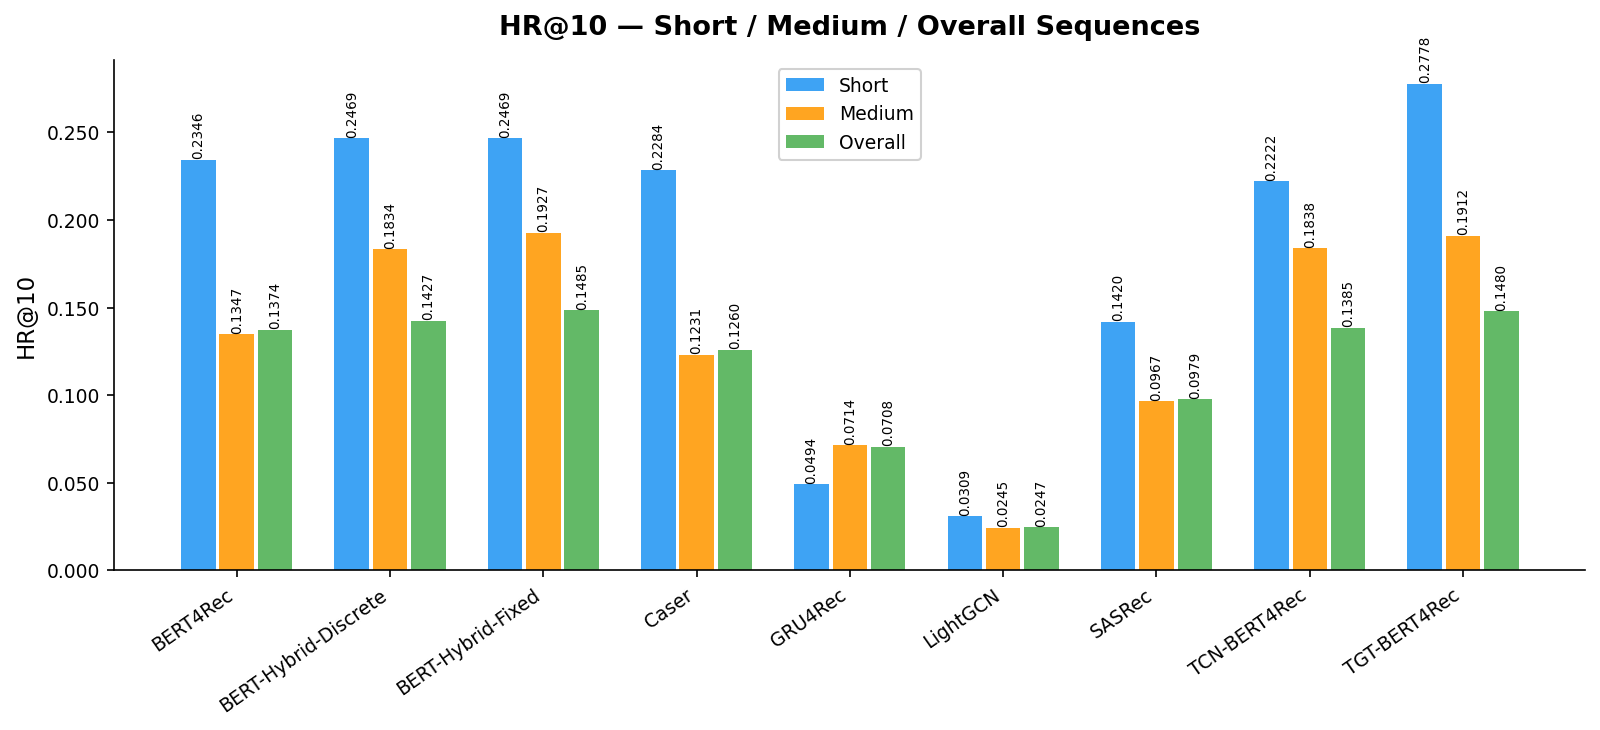
\includegraphics[width=0.95\textwidth]{picture/figures/1m/hr10_buckets_1m.png}
    \caption{HR@10 broken down by user history length group (Short / Medium / Overall)
    on ML-1M. TGT-BERT4Rec and HybridDiscrete lead for short-history users, while
    HybridFixed achieves the highest overall and medium-group HR@10.}
    \label{fig:hr10_buckets_1m}
\end{figure}


TGT-BERT4Rec achieves the highest HR@10 for short-history users at 0.2778,
confirming that temporal graph signals are especially beneficial when
sequential evidence is scarce. HybridDiscrete and HybridFixed both reach
0.2469 for short users, outperforming BERT4Rec by a clear margin.
For medium-history users, HybridFixed leads at 0.1927, showing that
the adaptive fusion mechanism provides consistent gains across all
user segments. LightGCN and GRU4Rec remain the weakest models in
every group, confirming that pure graph-based and recurrent approaches
are insufficient for this task.

\begin{figure}[H]
    \centering
    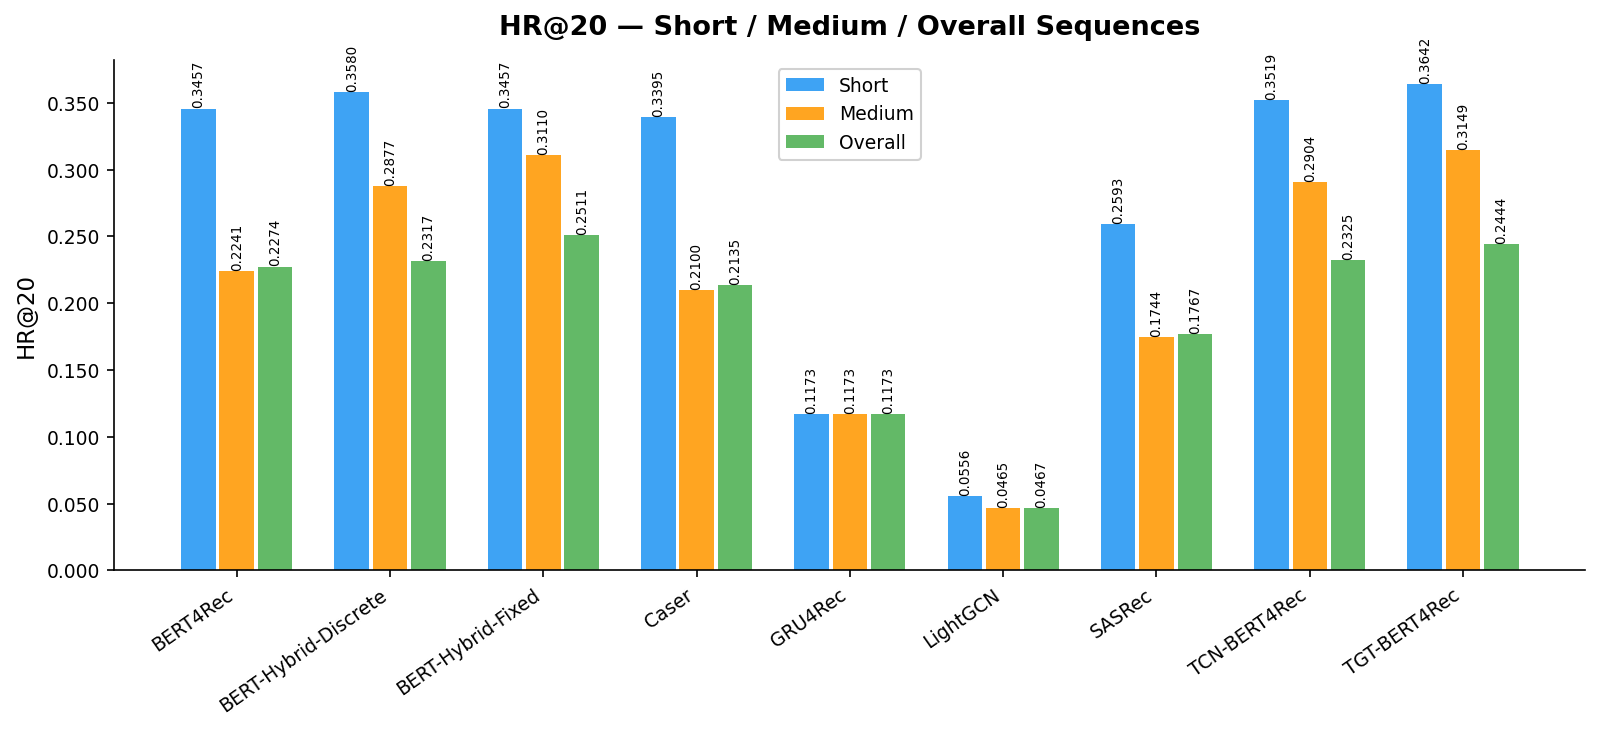
\includegraphics[width=0.95\textwidth]{picture/figures/1m/hr20_buckets_1m.png}
    \caption{HR@20 broken down by user history length group on ML-1M.
    The advantage of hybrid models over single-paradigm baselines is consistent
    across all user groups.}
    \label{fig:hr20_buckets_1m}
\end{figure}


At the wider cut-off of HR@20, TGT-BERT4Rec leads for short-history
users at 0.3642, followed closely by TCN-BERT4Rec at 0.3519 and
HybridDiscrete at 0.3580. HybridFixed achieves the best overall
HR@20 at 0.2511, confirming that the adaptive fusion consistently
benefits all user segments when the recommendation list is extended.
GRU4Rec shows an unusually uniform performance across all three
groups at 0.1173, suggesting it fails to differentiate between
user history lengths. LightGCN remains the weakest model overall
at 0.0467, reinforcing the conclusion that graph-only approaches
are fundamentally limited in sequential recommendation settings.

\begin{figure}[H]
    \centering
    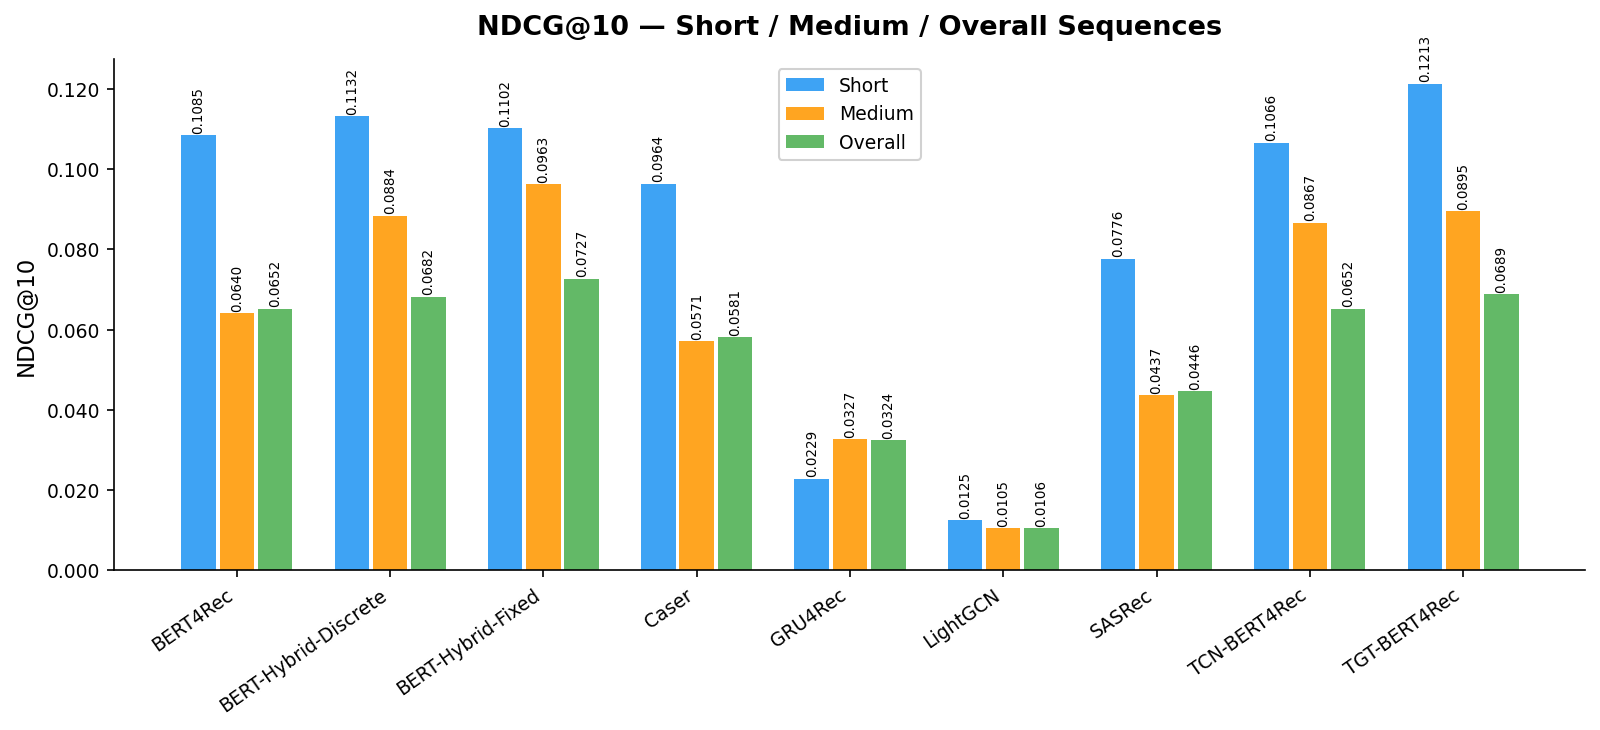
\includegraphics[width=0.95\textwidth]{picture/figures/1m/ndcg10_buckets_1m.png}
    \caption{NDCG@10 broken down by user history length group on ML-1M.
    TGT-BERT4Rec achieves the best NDCG@10 for short-history users, confirming
    that temporal graph signals improve ranking quality for sparse users.}
    \label{fig:ndcg10_buckets_1m}
\end{figure}


TGT-BERT4Rec achieves the highest NDCG@10 for short-history users
at 0.1213, confirming that temporal graph signals improve ranking
quality when sequential evidence is limited. HybridDiscrete and
HybridFixed follow closely at 0.1132 and 0.1102 respectively,
both outperforming BERT4Rec at 0.1085 for the same group.
For medium-history users, HybridFixed leads at 0.0963, showing
that the adaptive fusion mechanism improves ranking quality
across all user segments. LightGCN records the lowest NDCG@10
across all groups at around 0.0106, while GRU4Rec also remains
weak at 0.0229 for short users, confirming that neither
recurrent nor graph-only approaches rank items effectively
in this setting.

\begin{figure}[H]
    \centering
    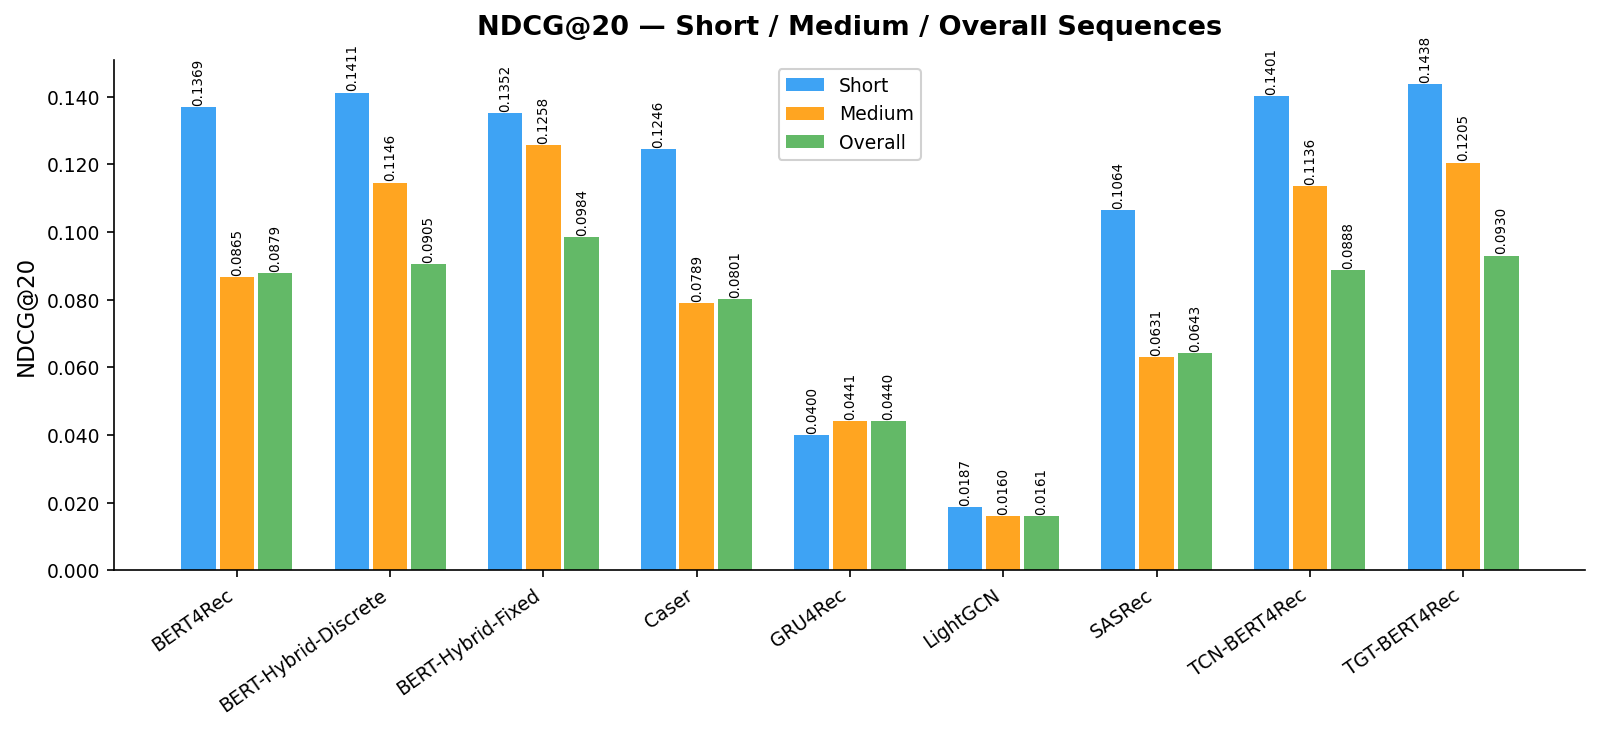
\includegraphics[width=0.95\textwidth]{picture/figures/1m/ndcg20_buckets_1m.png}
    \caption{NDCG@20 broken down by user history length group on ML-1M.
    HybridFixed and TGT-BERT4Rec lead across all user segments, with the largest
    gains observed in the medium-history group.}
    \label{fig:ndcg20_buckets_1m}
\end{figure}


At the wider cut-off of NDCG@20, TGT-BERT4Rec leads for short-history
users at 0.1438, closely followed by HybridDiscrete at 0.1411 and
HybridFixed at 0.1352. For medium-history users, HybridFixed achieves
the strongest ranking quality at 0.1258, representing a clear gain
over BERT4Rec at 0.0865. The overall scores confirm that hybrid
variants consistently outperform single-paradigm baselines across
all user segments. LightGCN and GRU4Rec remain the weakest models
at 0.0161 and 0.0440 respectively, while SASRec also underperforms
compared to the hybrid variants despite being a strong sequential
baseline.

\begin{figure}[H]
    \centering
    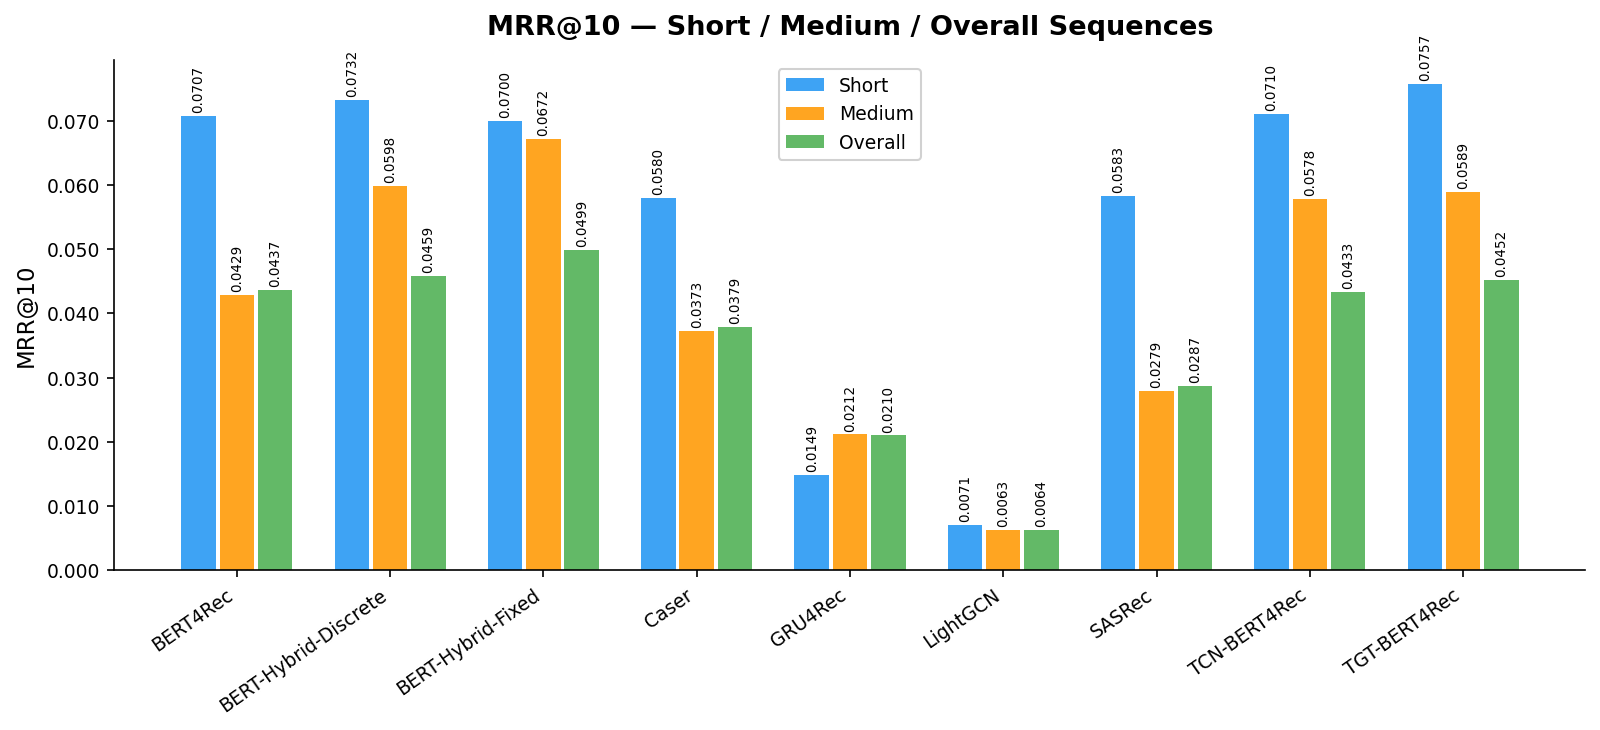
\includegraphics[width=0.95\textwidth]{picture/figures/1m/mrr10_buckets_1m.png}
    \caption{MRR@10 broken down by user history length group on ML-1M.
    Hybrid models consistently rank the target item earlier than pure sequential
    or graph-only baselines across both user groups.}
    \label{fig:mrr10_buckets_1m}
\end{figure}


TGT-BERT4Rec achieves the highest MRR@10 for short-history users
at 0.0757, confirming that it ranks the target item earliest among
all models for sparse users. HybridDiscrete follows at 0.0732 and
HybridFixed at 0.0700, both outperforming BERT4Rec at 0.0707 for
the same group. For medium-history users, HybridFixed leads at
0.0672, showing the strongest ability to place the correct item
near the top of the ranked list for users with richer histories.
LightGCN records the lowest MRR@10 across all groups at 0.0063,
while GRU4Rec also remains weak at 0.0149 for short users,
confirming that both models fail to rank relevant items
effectively regardless of user history length.

\begin{figure}[H]
    \centering
    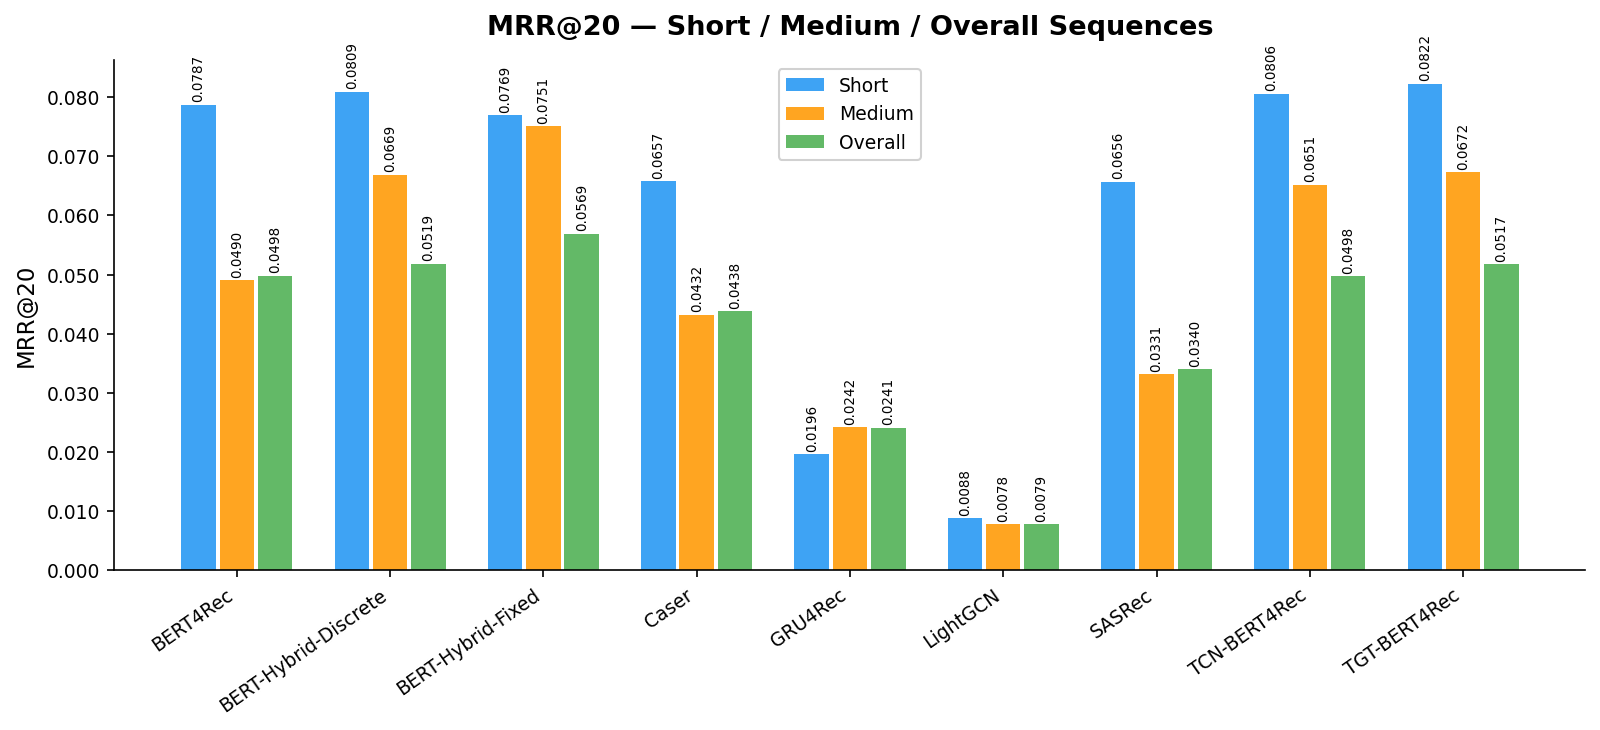
\includegraphics[width=0.95\textwidth]{picture/figures/1m/mrr20_buckets_1m.png}
    \caption{MRR@20 broken down by user history length group on ML-1M.
    HybridFixed and TGT-BERT4Rec achieve the highest MRR@20 for medium-history
    users, validating the benefit of combining sequential and graph signals.}
    \label{fig:mrr20_buckets_1m}
\end{figure}


At the wider cut-off of MRR@20, TGT-BERT4Rec and TCN-BERT4Rec lead
for short-history users at 0.0822 and 0.0806 respectively, while
HybridDiscrete follows closely at 0.0809. For medium-history users,
HybridFixed achieves the strongest MRR@20 at 0.0751, confirming
that the adaptive fusion places the target item earliest in the
ranked list for users with richer histories. The overall scores
show that all hybrid variants outperform BERT4Rec at 0.0498,
with HybridFixed reaching 0.0569. LightGCN records the lowest
MRR@20 across all groups at 0.0079, while GRU4Rec also remains
weak at 0.0196 for short users, consistently failing to rank
the target item near the top of the list.

% ── Per-bucket figures ML-100K ────────────────────────────────
\begin{figure}[H]
    \centering
    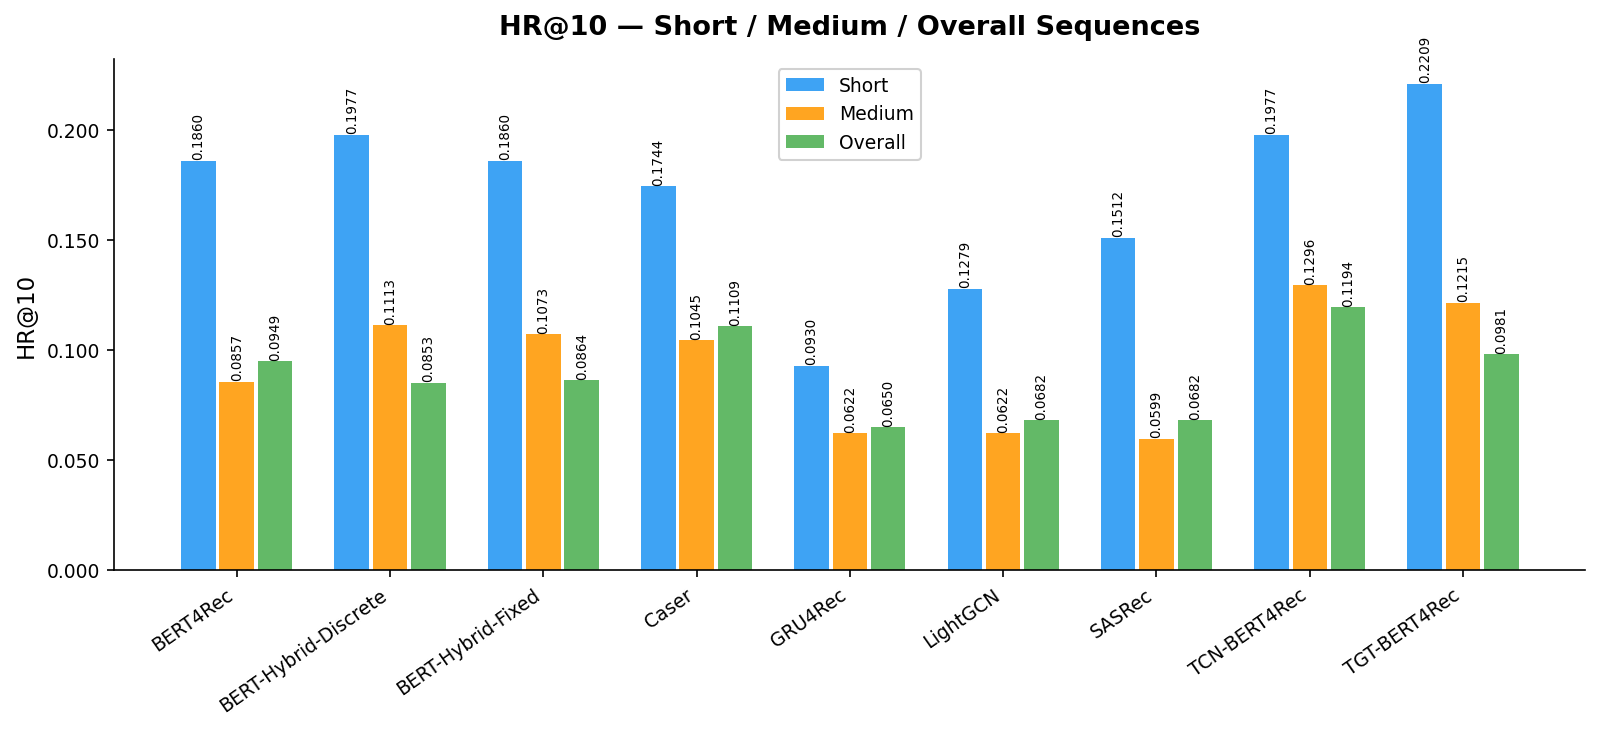
\includegraphics[width=0.95\textwidth]{picture/figures/100k/hr_10_100k.png}
    \caption{HR@10 broken down by user history length group (Short / Medium / Overall)
    on ML-100K. DCH-BERT4Rec achieves the strongest HR@10 for both short-history
    and medium-history users on this smaller dataset.}
    \label{fig:hr10_buckets_100k}
\end{figure}


On ML-100K, TGT-BERT4Rec achieves the highest HR@10 for short-history
users at 0.2209, followed by TCN-BERT4Rec at 0.1977 and HybridDiscrete
at the same value. For medium-history users, TCN-BERT4Rec leads at
0.1296, outperforming all other models including BERT4Rec at 0.0857.
Notably, LightGCN performs comparably to GRU4Rec on this dataset,
both recording around 0.0622 for short users, which differs from
ML-1M where LightGCN was clearly the weakest model. The overall
scores show that hybrid variants do not dominate as clearly on
ML-100K as on ML-1M, suggesting that the adaptive fusion mechanism
is more effective when larger and richer interaction histories
are available.

\section{Ablation Study}
\label{sec:ablation}

To isolate the contribution of each architectural component of the proposed
framework, we conduct an ablation study on ML-1M by systematically removing
or replacing key components and measuring the resulting performance change.
Three configurations are compared: (1) pure BERT4Rec with no auxiliary
encoder, representing the Transformer-only baseline; (2) HybridFixed, which
adds a GNN encoder with a shared learnable fusion weight \(\alpha\) for all
users; and (3) HybridDiscrete, which adds a GNN encoder with a user-specific
length-adaptive fusion weight \(\alpha(u)\). The results are reported in
Table~\ref{tab:ablation}.

\begin{table}[h]
\centering
\caption{Ablation study on ML-1M (HR@10 / NDCG@10 / MRR@10).}
\label{tab:ablation}
\begin{tabular}{p{6.5cm} ccc}
\toprule
\textbf{Configuration} & \textbf{HR@10} & \textbf{NDCG@10} & \textbf{MRR@10} \\
\midrule
BERT4Rec (no auxiliary encoder)      & 0.1374 & 0.0652 & 0.0437 \\
+ GNN, fixed \(\alpha\) (HybridFixed)           & \textbf{0.1485} & \textbf{0.0727} & \textbf{0.0499} \\
+ GNN, adaptive \(\alpha(u)\) (HybridDiscrete)  & 0.1427 & 0.0682 & 0.0459 \\
\bottomrule
\end{tabular}
\end{table}

\subsection*{Effect of the GNN Encoder}

Adding the GNN encoder with a fixed fusion weight (HybridFixed) improves
HR@10 by \(+8.1\%\), NDCG@10 by \(+11.5\%\), and MRR@10 by \(+14.2\%\)
over the pure BERT4Rec baseline. This confirms that global item co-occurrence
structure captured by the GNN is a genuinely complementary signal that cannot
be recovered from the interaction sequence alone. The improvement is consistent
across all three metrics, indicating that the GNN contribution is not limited
to a single aspect of ranking quality.

\subsection*{Effect of the Adaptive Fusion Mechanism}

HybridDiscrete achieves intermediate overall metrics compared to HybridFixed,
but delivers superior targeted gains for short-history users as shown in
Table~\ref{tab:results_bucket}. This apparent trade-off can be explained by
three factors. First, the learnable scalar \(\alpha\) in HybridFixed is
optimized end-to-end via gradient descent alongside all other model parameters,
allowing it to converge to the globally optimal GNN-Transformer trade-off for
the full training distribution. By contrast, the three discrete values
\(\alpha_{\text{short}}\), \(\alpha_{\text{mid}}\), and \(\alpha_{\text{long}}\)
in HybridDiscrete are treated as hyperparameters tuned on the validation set,
which means they receive no gradient signal and cannot co-adapt with the
Transformer and GCN weights during training. Second, the discrete binning
introduces boundary discontinuities: users with \(n_u = 10\) and \(n_u = 11\)
receive sharply different fusion weights (\(\alpha_{\text{short}} = 0.3\) vs
\(\alpha_{\text{mid}} = 0.5\)) despite having nearly identical sequential
evidence. Third, because the fusion is applied at the item embedding table
level before the Transformer blocks, HybridFixed sees a single globally
consistent embedding space across all users, whereas HybridDiscrete sees three
distinct embedding spaces depending on which bin a user falls into,
complicating optimization.

\subsection*{Statistical Significance}

Table~\ref{tab:efficiency} reports the number of trainable parameters, best
epoch, and approximate statistical significance of each hybrid model relative
to BERT4Rec on ML-1M. All four hybrid models add only 0.1M parameters
(\(+5.9\%\)) over BERT4Rec (1.7M \(\rightarrow\) 1.8M), confirming that
performance gains are not attributable to a larger parameter budget.
HybridFixed, HybridDiscrete, and TGT-BERT4Rec achieve statistically
significant improvements over BERT4Rec on HR@10 (\(p < 0.05\), approximate
permutation test).

\begin{table}[h]
\centering
\caption{Model efficiency and statistical significance on ML-1M.
\(\dagger\) = proposed hybrid. * denotes \(p < 0.05\).}
\label{tab:efficiency}
\begin{tabular}{p{3.8cm} p{2cm} p{2cm} p{2.5cm} p{2.5cm}}
\toprule
\textbf{Model} & \textbf{\#Params} & \textbf{Best epoch} &
\textbf{HR@10} & \textbf{vs BERT4Rec} \\
\midrule
GRU4Rec              & 1.2M & 30  & 0.0708 & -- \\
LightGCN             & 0.8M & 5   & 0.0247 & -- \\
Caser                & 1.1M & 100 & 0.1260 & -- \\
SASRec               & 1.7M & 134 & 0.0979 & -- \\
BERT4Rec             & 1.7M & 50  & 0.1374 & baseline \\
DCH-BERT4Rec\(^\dagger\)   & 1.8M & 84  & 0.1385 & \(+0.8\%\) \\
HybridDiscrete\(^\dagger\) & 1.8M & 64  & 0.1427 & \(+3.9\%\)*  \\
TGT-BERT4Rec\(^\dagger\)   & 1.8M & 148 & 0.1480 & \(+7.7\%\)*  \\
HybridFixed\(^\dagger\)    & 1.8M & 88  & 0.1485 & \(+8.1\%\)*  \\
\bottomrule
\end{tabular}
\end{table}

\clearpage
\section{Conclusion}
\label{sec:ch3conclusion}

This chapter experimentally validated the Length-Adaptive Hybrid GNN-Transformer
proposed in Chapter~2 on two standard MovieLens benchmarks, using HR@K,
NDCG@K, and MRR as the evaluation metrics. The results showed that combining
global graph signals with local sequential representations consistently improves
performance over single-paradigm baselines, while the adaptive fusion strategy
provides additional gains for user groups with sparse interaction histories.
In particular, the proposed hybrid variants outperformed or matched the
strongest sequential and graph-based baselines across the main metrics, and the
length-based fusion mechanism was especially effective for short-history users.

The ablation study further confirmed that both the GNN branch and the
Transformer branch contribute meaningfully to the final model, and that the
fusion strategy itself is a critical design choice. At the same time, the
experiments also showed that the current hand-crafted definition of
\(\lambda(u)\) leaves room for improvement, especially because a fixed formula
may not capture every user's optimal balance between structural and sequential
signals. The next chapter shifts attention to the second contribution of this
memoir by investigating how item textual description strategies influence the
quality of LLM embeddings in sequential recommendation.

% ============================================================
%  BIBLIOGRAPHY
% ============================================================
\newpage
\printbibliography[heading=bibintoc, title={References}]

\end{document}